\chapter{Series}

\section{Sucesiones numéricas}

\begin{defi}
Una \textbf{sucesión} de números complejos es una función del tipo
$$f: \mathbb{N} \rightarrow \mathbb{C}, \quad n \mapsto f(z) = z_n.$$
\end{defi}

\textbf{Observación:} Su recorrido es 
$$\{z_n : n \in \mathbb{N}\} = \{z_1, z_2, \dots, z_n\}.$$

Con el fin de simplificar las notaciones, denotaremos una sucesión simplemente por 
$$\{z_n\}_{n\in \mathbb{N}}, ~ \{z_n\}_{n=1}^{\infty}, ~ \{z_n\}_{n=m}^{\infty}, ~ etc.$$

\begin{defi}
Se dice que una sucesión $\{z_n\}_{n=1}^{\infty}$ \textbf{converge} a $z \in \mathbb{C}$ si
$$(\forall \varepsilon > 0)(\exists N \in \mathbb{N})(\forall n: ~ n \geq N \Rightarrow |z_n - z| < \varepsilon).$$

Ésto se denotará por
$$\lim_{n\to +\infty} z_n = z$$

y $z$ se llamará límite de la sucesión $\{z_n\}_{n=1}^{\infty}$. Si no existe tal $z \in \mathbb{C}$ diremos que $\{z_n\}_{n=1}^{\infty}$ \textbf{diverge}.
\end{defi}

\begin{figure}[H]
    \centering
    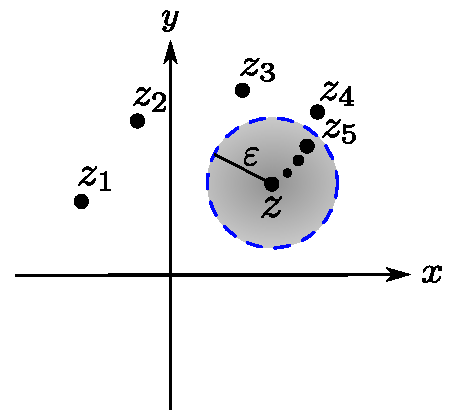
\includegraphics[scale = 0.7]{Figuras/ConvergenciaSucesion.pdf}
    \caption{Sucesión $\{z_n\}_{n\in \mathbb{N}}$ convergiendo a $z$.}
    \label{fig:Sucesion}
\end{figure}

Para sucesiones que convergen a cero, es fácil de ver que
$$\lim_{n\to + \infty} z_n = 0 \Leftrightarrow \lim_{n \to + \infty} |z_n| = 0.$$

Note que las definiciones son similares al de las sucesiones reales, por tanto se omitirán las demostraciones que sean similares al caso real.

\begin{propo}
Si el límite de una sucesión compleja existe, entonces éste es único.
\end{propo}

\begin{teorema} \label{SucesionCom-Re}
Sea $\{z_n\}_{n \in \mathbb{N}}$ una sucesión de números complejos tal que $z_n = x_n + iy_n$, donde $x_n=Re(z_n)$ e $y_n = Im(z_n)$. Entonces, para $z = x + iy$, tenemos
$$\lim_{n\to + \infty} z_n = z \Leftrightarrow \lim_{n\to + \infty} x_n = x ~\wedge~ \lim_{n\to + \infty} y_n = y.$$
\end{teorema}

\begin{proof}
Supongamos que $\lim\limits_{n\to + \infty} z_n = z$, entonces dado $\varepsilon >0 $, $\exists N \in \mathbb{N}$ tal que 
$$\forall n: ~ n \geq N \Rightarrow |z_n-z| = |(x_n-x) + i (y_n-y)| < \varepsilon.$$

Usando el mismo $N \in \mathbb{N}$, se verifica:
\begin{align*}
    \forall n:~ n \geq N &\Rightarrow |x_n-x| \leq  |(x_n-x) + i (y_n-y)| < \varepsilon, \\
    \forall n:~ n \geq N & \Rightarrow |y_n-y| \leq  |(x_n-x) + i (y_n-y)| < \varepsilon.
\end{align*}

Por lo tanto,
$$\lim_{n\to + \infty} x_n = x \wedge \lim_{n\to + \infty} y_n = y.$$

Por otro lado, supongamos que $\lim\limits_{n\to + \infty} x_n = x$ y $\lim\limits_{n\to + \infty} y_n = y$, entonces dado $\varepsilon > 0$, $\exists N_1, N_2 \in \mathbb{N}$ tales que
\begin{align*}
    \forall n:~ n \geq N_1 &\Rightarrow |x_n-x|  < \frac{\varepsilon}{2}, \\
    \forall n:~ n \geq N_2 &\Rightarrow |y_n-y| < \frac{\varepsilon}{2}.
\end{align*}

Eligiendo $N = \max\{N_1, N_2\}$, se verifica:
\begin{align*}
    \forall n: ~ n\geq N \Rightarrow |z_n-z| &=  |(x_n-x) + i (y_n-y)| \\
    &\leq |x_n-x| + |y_n-y| \\
    &< \frac{\varepsilon}{2} + \frac{\varepsilon}{2} = \varepsilon.
\end{align*}

Por lo tanto, 
$$\lim_{n\to + \infty} z_n = z.$$
\end{proof}

\begin{ejemplo}
Estudiar el comportamiento de la sucesión $\{(i)^n\}_{n \in \mathbb{N}}$.
\\

\textbf{Solución:} Consideremos las siguientes subsucesiones: $\left\{ (i)^{4k-2}\right\}_{k \in \mathbb{N}}$ y $\left\{ (i)^{4k}\right\}_{k \in \mathbb{N}}$. Luego,
\begin{align*}
    \lim_{k \to + \infty} (i)^{4k-2} &= \lim_{k \to + \infty} (-1) = -1, \\
    \lim_{k \to + \infty} (i)^{4k} &= \lim_{k \to + \infty} 1 = 1.
\end{align*}

Como $\lim\limits_{k \to + \infty} i^{4k-2} \neq \lim\limits_{k \to + \infty} i^{4k}$, la sucesión $\{(i)^n\}_{n \in \mathbb{N}}$ diverge.
\end{ejemplo}

\begin{defi}
Una sucesión de números complejos $\{z_n\}_{n=1}^{\infty}$ se dice que es \textbf{acotada} si existe $M > 0$ tal que 
$$\forall n \in \mathbb{N}: ~ |z_n| \leq M.$$
\end{defi}

\begin{teorema}
Toda sucesión de números complejos convergente es acotada.
\end{teorema}

\textbf{Observación:} El recíproco es falso, pues la sucesión $\{(i)^n\}_{n \in \mathbb{N}}$ es acotada pero no converge.

\begin{teorema}
Sean $\{z_n\}_{n\in \mathbb{N}}$ y $\{w_n\}_{n\in \mathbb{N}}$  sucesiones de números complejos.
\begin{itemize}
    \item[(i)] Si $\lim\limits_{n\to + \infty} z_n = 0$ y $|w_n| \leq |z_n|$ para todo $n \geq N_0 \in \mathbb{N}$. Entonces, $\lim\limits_{n\to + \infty} w_n = 0$.
    
    \item[(ii)] Si  $\lim\limits_{n\to + \infty} z_n = 0$ y $\{w_n\}_{n\in \mathbb{N}}$ es acotada, entonces  $\lim\limits_{n\to + \infty} z_n w_n = 0$.
\end{itemize}
\end{teorema}

\begin{teorema}[Álgebra de límites]
Sean $\{z_n\}_{n\in \mathbb{N}}$ y $\{w_n\}_{n\in \mathbb{N}}$  dos sucesiones de números complejos convergentes y $\alpha,\beta \in \mathbb{C}$. Entonces
\begin{itemize}
\item[(i)] $$\lim\limits_{n \to + \infty} (\alpha z_n + \beta w_n ) = \alpha \lim\limits_{n\to + \infty} z_n + \beta \lim\limits_{n\to + \infty} w_n;$$

\item[(ii)] $$\lim\limits_{n \to + \infty} ( z_n w_n) = \left( \lim\limits_{n\to + \infty} z_n\right) \cdot \left(\lim\limits_{n\to + \infty} w_n \right);$$

\item[(iii)] $$\lim\limits_{n \to + \infty} \frac{z_n}{w_n} = \frac{\lim\limits_{n\to + \infty} z_n}{\lim\limits_{n\to + \infty} w_n}, \quad \mbox{cuando} ~\lim\limits_{n\to + \infty} w_n \neq 0;$$

\item[(iv)] $$\lim\limits_{n \to + \infty} \overline{z_n} = \overline{\lim\limits_{n\to + \infty} z_n};$$

\item[(v)] $$\lim\limits_{n\to + \infty} |z_n| = \left| \lim\limits_{n\to + \infty} z_n\right|.$$
\end{itemize}
\end{teorema}

\begin{ejemplo} \label{EjemploSucesion}
Muestre que
$$\lim_{n\to + \infty} z^n = \left\{ \begin{array}{cl}
    0,& \mbox{si} ~ |z| < 1  \\
    1, &  \mbox{si} ~ z = 1 \\
    diverge, &\mbox{si} ~ |z| = 1 \wedge z \neq 1 \\
    diverge, &\mbox{si} ~ |z| > 1
\end{array} \right. .$$

\textbf{Solución:} Recordemos que para un número real $r \geq 0$, tenemos
$$\lim_{n\to + \infty} r^n = \left\{ \begin{array}{cl}
    0,& \mbox{si} ~ 0\leq r < 1  \\
    1, &  \mbox{si} ~ r = 1 \\
    \infty, &\mbox{si} ~ r > 1
\end{array} \right. .$$


En consecuencia, para un número complejo $|z| < 1$, tenemos 
$$\lim_{n\to + \infty} |z|^n = \lim_{n\to + \infty} |z^n| =   0 \Rightarrow  \lim_{n\to + \infty} z^n = 0.$$

Para $|z| > 1$, tenemos que 
$$\lim_{n\to + \infty} |z|^n = + \infty,$$

ésto es, $\{z_n\}_{n = 1}^{\infty}$ no es acotada. Luego, no converge. 

Ahora, para $|z| = 1$, es trivial que si $z = 1$ la sucesión converge. El caso $|z| = 1$, $z\neq 1$, no es tan simple, pues la sucesión está acotada. Supongamos que la serie converge, es decir,
$$\lim_{n\to + \infty} z^n = L \in \mathbb{C} \Rightarrow |L| = \lim_{n\to + \infty} |z|^n = 1,$$

así $L \neq 0$. Además, si $z^n \to L$, entonces $z^{n+1} \to L$ cuando $n\to + \infty$. Pero 
$$L = \lim_{n\to + \infty} z^{n+1} = \lim_{n\to + \infty} z^{n}z = Lz.$$

Dividiendo por $L$, deducimos que $z = 1$, lo cual es una contradicción, pues $|z| =1$ con $z \neq 1$. Por lo tanto, la sucesión diverge.
\end{ejemplo}

Antes de finalizar la sección, estudiemos la completitud de $\mathbb{C}$, ésto es, si las \textit{sucesiones de Cauchy} convergen. Para ello, recordemos que son estas sucesiones.

\begin{defi}
Una sucesión $\{z_n\}_{n=1}^{\infty}$ se dice que es una \textbf{sucesión de Cauchy} si para cada $\varepsilon > 0$, existe $N \in \mathbb{N}$ tal que
$$\forall n,m:~ n,m \geq N \Rightarrow |z_n-z_m| < \varepsilon.$$
\end{defi}

Utilizando como hecho la completitud de los reales, podemos probar el siguiente teorema.

\begin{teorema}
Una sucesión $\{z_n\}_{n=1}^{\infty}$ de números complejos converge si y sólo si es una sucesión de Cauchy.
\end{teorema}

\begin{proof}
Supongamos que $\{z_n\}_{n=1}^{\infty}$ converge a $z \in \mathbb{C}$, entonces dado $\varepsilon >0$, $\exists N \in \mathbb{N}$ tal que
$$\forall n:~ n \geq N ~\Rightarrow~ |z_n - z| < \frac{\varepsilon}{2}.$$

Sean $n,m \geq N$, se cumple
$$|z_n - z_m| = |(z_n - z) + (z - z_m)| \leq |z_n -z| + |z_m - z| < \varepsilon.$$

Por lo tanto, $\{z_n\}_{n=1}^{\infty}$ es de Cauchy, probando así la implicancia hacia la derecha.
\\

Por otro lado, supongamos que $\{z_n\}_{n=1}^{\infty}$ es una sucesión de Cauchy, entonces
$$(\forall \varepsilon > 0)(\exists N \in \mathbb{N})(\forall n,m: ~ n,m \geq N ~\Rightarrow~ |z_n-z_m| < \varepsilon)$$

Si $z_n = x_n + iy_n$, entonces
$$|x_n - x_m| < \varepsilon ~\wedge~ |y_n - y_m| < \varepsilon, \quad \forall n,m \geq N.$$

Ésto es, las sucesiones $\{x_n\}_{n=1}^{\infty}$ y  $\{y_n\}_{n=1}^{\infty}$  son de Cauchy en $\mathbb{R}$ y en consecuencia convergen. Finalmente, por el teorema \ref{SucesionCom-Re}, la sucesión $\{z_n\}_{n=1}^{\infty}$ converge, probando así la implicancia hacia la izquierda.
\end{proof}

\section{Series numéricas}

\begin{defi}
Sea $\{z_n\}_{n=1}^{\infty}$ una sucesión de números complejos. Se define la sucesión de \textbf{sumas parciales}  $\{s_n\}_{n=1}^{\infty}$ por 
\begin{align*}
    s_1 &= z_1 \\
    s_2 &= s_1 + z_2 = z_1+ z_2 \\
    s_3 &= s_2 + z_3 = z_1 + z_2 + z_3 \\
    &~\,\vdots \\
    s_n &= s_{n-1} + z_n = z_1 + z_2 + z_3 + \cdots + z_n.
\end{align*}

Esta nueva sucesión recibe el nombre de \textbf{serie} de término general $z_n$ y se denota
$$\sum_{n=1}^{\infty} z_n.$$

Si la sucesión de sumas parciales $\{s_n\}_{n=1}^{\infty}$ converge al valor $S$, se dice que la serie es convergente y se escribe
$$\sum_{n=1}^{\infty} z_n = S.$$

El número $S$ se llama \textbf{suma} de la serie. Si   $\{s_n\}_{n=1}^{\infty}$ diverge, se dice que la serie diverge.
\end{defi}

\begin{ejemplo} \label{SerieGeo}
Muestre que si $|z| < 1$, la \textbf{serie geométrica} $\sum\limits_{n=0}^{\infty} z^n$ converge y
$$\sum_{n=0}^{\infty} z^n = \frac{1}{1-z}.$$

Muestre también que la serie diverge para los otros valores de $z$.
\\

\textbf{Solución:} 

Para $z=1$, la $n$-ésima suma parcial es $s_n = n$ y por tanto la serie diverge.

Para $z\neq 1$, la $n$-ésima suma parcial es
\begin{equation}
    s_n = \sum_{k=0}^n z^k = 1 + z +z^2 + \cdots + z^n. \label{Geometrica1}
\end{equation}

Multiplicando por $z$:
\begin{equation}
    z s_n = \sum_{k=0}^n z^{k+1} = z + z^2  + \cdots + z^n + z^{n+1}. \label{Geometrica2}
\end{equation}

Entonces, tomando la diferencia entre \eqref{Geometrica1} y \eqref{Geometrica2}, tenemos
$$(1-z) s_n = \sum_{k=0}^n [z^k - z^{k+1}] = 1 - z^{n+1} ~\Rightarrow~ s_n = \frac{1-z^{n+1}}{1-z}.$$

Por el ejemplo \ref{EjemploSucesion}, tenemos que $\{z^{n+1}\}_{n=0}^{\infty}$ converge a 0 si $|z|<1$ y diverge si $|z| > 1$ o $|z|=1$ y $z \neq 1$. Esto implica que
$$\sum_{n=0}^{\infty} z^n = \frac{1}{1-z}, \quad |z| <1.$$
\end{ejemplo}
\newpage

Al igual que en el caso de las sucesiones, se omitirán las demostraciones que son análogas al caso real.

\begin{teorema} \label{SerieCom-Re}
Sea $\sum\limits_{n=1}^{\infty} z_n$ una serie de números complejos tal que $z_n = x_n + iy_n$, donde $x_n=Re(z_n)$ e $y_n = Im(z_n)$. Entonces, para $S = x + iy$, tenemos
$$\sum_{n=1}^{\infty} z_n = S \Leftrightarrow \sum_{n=1}^{\infty} x_n = x ~\wedge~ \sum_{n=1}^{\infty} y_n = y.$$
\end{teorema}

\begin{proof}
Sea $S_n$ la $n$-ésima suma parcial de la serie $\sum\limits_{n=1}^{\infty} z_n$, observemos que
$$S_n = X_n + i Y_n,$$

donde
$$X_n = \sum_{k=1}^n x_n ~~\mbox{y}~~ Y_n = \sum_{k=1}^n y_n.$$

Ahora, por el teorema \ref{SucesionCom-Re}, 
$$\lim_{n \to + \infty} S_n = S \Leftrightarrow \lim_{n \to \infty} X_n = x ~\wedge~ \lim_{n \to \infty} Y_n = y.$$

Como $X_n$ e $Y_n$ son las $n$-ésimas sumas parciales de las series $\sum\limits_{n=1}^{\infty} x_n$ y $\sum\limits_{n=1}^{\infty} y_n$, respectivamente. Queda demostrado el teorema.

\end{proof}

\begin{teorema}\label{AlgebraSeries}
Si $\sum\limits_{n=1}^{\infty} z_n$ y $\sum\limits_{n=1}^{\infty} w_n$ son series de números complejos convergentes, y $\alpha,\beta \in \mathbb{C}$. Entonces,
\begin{itemize}
    \item[(i)] $\sum\limits_{n=1}^{\infty} (\alpha z_n + \beta w_n) = \alpha \sum\limits_{n=1}^{\infty} z_n + \beta \sum\limits_{n=1}^{\infty} w_n;$
    
    \item[(ii)] $\overline{\sum\limits_{n=1}^{\infty} z_n} =  \sum\limits_{n=1}^{\infty} \overline{z_n};$
    
    \item[(iii)] $Re\left(\sum\limits_{n=1}^{\infty} z_n\right) =\sum\limits_{n=1}^{\infty} Re(z_n)$ y $Im\left(\sum\limits_{n=1}^{\infty} z_n\right) =\sum\limits_{n=1}^{\infty} Im(z_n)$
\end{itemize}
\end{teorema}

En el siguiente ejemplo se ilustra como podemos usar series complejas para determinar una serie real.

\begin{ejemplo}
Mostrar que 
$$\sum_{n=0}^{\infty} \frac{\cos(n\theta)}{2^n}$$

converge para todo $\theta$ y encontrar la suma.
\\

\textbf{Solución:} Notemos que $\cos(n\theta)$ es la parte real de $(\cos\theta + i \sin \theta)^n$, entonces la serie dada es la parte real de la serie geométrica
$$\sum_{n=0}^{\infty} z^n, \quad \mbox{donde} ~ z = \frac{1}{2}(\cos \theta + i \sin \theta).$$

Como $|z| = 1/2 < 1$, tenemos que la serie converge y
\begin{align*}
 \sum_{n=0}^{\infty} z^n = \frac{1}{1-z} &= \frac{1}{\left(1 - \frac{1}{2} \cos \theta \right) - \frac{i}{2} \sin \theta } \cdot \frac{\left(1 - \frac{1}{2} \cos \theta \right) + \frac{i}{2} \sin \theta}{\left(1 - \frac{1}{2} \cos \theta \right) + \frac{i}{2} \sin \theta} \\
 &= \frac{1 - \frac{1}{2} \cos \theta  + \frac{i}{2} \sin \theta}{\left(1 - \frac{1}{2} \cos \theta \right)^2 + \left(\frac{1}{2} \sin \theta\right)^2} \\
 &= \frac{4-2\cos\theta+2i\sin\theta}{5-4\cos \theta}.
\end{align*}

Tomando las partes reales y usando el teorema \ref{AlgebraSeries} (iii), obtenemos 
$$\sum_{n=0}^{\infty} \frac{\cos(n\theta)}{2^n} = Re\left( \frac{4-2\cos\theta+2i\sin\theta}{5-4\cos \theta}\right) = \frac{4-2\cos \theta}{5-4\cos \theta}, \quad \forall\theta\in \mathbb{R}.$$
\end{ejemplo}

\begin{propo}
Si la serie $\sum\limits_{n=1}^{\infty} z_n$ es convergente, entonces $\lim\limits_{n\to + \infty} z_n = 0.$
\end{propo}

En la práctica, el contrarrecíproco es más útil:
$$\lim_{n\to + \infty} z_n \neq 0 ~\Rightarrow~ \sum_{n=1}^{\infty} z_n ~ \mbox{es divergente}.$$

\begin{defi}
Sea $\sum\limits_{n=1}^{\infty } z_n$ una serie de números complejos. Diremos que  $\sum\limits_{n=1}^{\infty } z_n$ \textbf{converge absolutamente} si $\sum\limits_{n=1}^{\infty} |z_n|$ converge. 
\end{defi}

\begin{teorema} \label{CVAbsoluta}
Las series absolutamente convergentes son convergentes, es decir, para $z_n \in \mathbb{C}$,
$$\sum_{n=1}^{\infty} |z_n| < \infty \Rightarrow \sum_{n=1}^{\infty} z_n ~\mbox{converge}.$$
\end{teorema}

\begin{proof}
Si $z_n = x_n + iy_n$, por hipótesis, la serie
$$\sum_{n=1}^{\infty} |z_n| = \sum_{n=1}^{\infty} \sqrt{x_n^2 + y_n^2}$$

de números reales converge. Como
$$|x_n| \leq \sqrt{x_n^2 + y_n^2} ~~\mbox{y}~~ |y_n| \leq \sqrt{x_n^2 + y_n^2},$$

usando el criterio de comparación directa real, las dos series
$$\sum_{n=1}^{\infty} |x_n| ~~\mbox{y}~~ \sum_{n=1}^{\infty} |y_n|$$

convergen. Además, ya que la convergencia absoluta de una serie de números reales implica la convergencia de la propia serie, se sigue que 
$$\sum_{n=1}^{\infty} x_n  ~~\mbox{y}~~ \sum_{n=1}^{\infty} y_n$$

convergen y, en consecuencia, también lo hace $\sum\limits_{n=1}^{\infty} z_n$.
\end{proof}

La importancia de este teorema radica en que al ser $\sum\limits_{n=1}^{\infty} |z_n|$ una serie real, los criterios usuales para series reales que conocemos del cálculo, pueden ser utilizados. 

\begin{teorema}
Supongamos que $z_n$ son números complejos, $a_n$ son números reales, $|z_n| \leq  a_n$ para todo $n \geq N_0 \in \mathbb{N}$, y $\sum\limits_{n=1}^{\infty} a_n$ es convergente. Entonces, $\sum\limits_{n=1}^{\infty} z_n$ es absolutamente convergente.
\end{teorema}

\begin{proof}
Directo del criterio de comparación directa para series reales y el teorema \ref{CVAbsoluta}.
\end{proof}

\begin{ejemplo}
Estudie la convergencia de la serie
$$\sum_{n=0}^{\infty} \frac{2\cos(n\theta) + 2i \sin(n\theta)}{n^2+3}.$$

\textbf{Solución:} Notemos que
$$\forall n \in \mathbb{N}: ~ \left| \frac{2\cos(n\theta) + 2i \sin(n\theta)}{n^2+3} \right| = \frac{2|\cos(n\theta) + i \sin(n\theta)|}{n^2+3} \leq \frac{2}{n^2+3} \leq \frac{2}{n^2}.$$

Como la serie $\sum\limits_{n=1}^{\infty} \frac{2}{n^2}$ converge, la serie
$$\sum_{n=0}^{\infty} \frac{2\cos(n\theta) + 2i \sin(n\theta)}{n^2+3} ~ \mbox{converge}.$$
\end{ejemplo}

Los criterios del cociente y de la raíz también pueden ser aplicados como se ilustra en los siguientes teoremas.

\begin{teorema}[Criterio del cociente]
Sea $\{z_n\}_{n=1}^{\infty}$ una sucesión de números complejos no nulos y 
$$L = \lim_{n \to + \infty} \left|\frac{z_{n+1}}{z_n} \right|.$$

Entonces,
\begin{itemize}
\item[i)] $0\leq L < 1 ~\Rightarrow~ \sum\limits_{n=1}^{\infty} z_n$ es absolutamente convergente.

\item[ii)] $L > 1 ~\Rightarrow~ \sum\limits_{n=1}^{\infty} z_n $ es divergente. \qquad (también para $L = + \infty$)

\item[iii)] Para $L = 1$, el criterio no proporciona información.
\end{itemize} 
\end{teorema}

\begin{ejemplo}
La serie
$$\sum_{n=0}^{\infty} \frac{z^n}{n!}$$

converge absolutamente para todo $z \in \mathbb{C}$. En efecto, la serie claramente converge si $z = 0$. Para $z \neq 0$,
$$L = \lim_{n\to + \infty} \left| \frac{z^{n+1}n!}{z^n (n+1)!} \right| = \lim_{n\to + \infty} \frac{|z|}{n+1} = 0.$$

Como $L < 1$, la serie converge absolutamente por el criterio del cociente.
\end{ejemplo}

\begin{teorema}[Criterio de la raíz]
Sea $\{z_n\}_{n=1}^{\infty}$ una sucesión de números complejos y 
$$L = \lim_{n \to + \infty} \sqrt[n]{|z_n|}.$$

Entonces,
\begin{itemize}
\item[i)] $0\leq L < 1 ~\Rightarrow~ \sum\limits_{n=1}^{\infty} z_n$ es absolutamente convergente.

\item[ii)] $L > 1 ~\Rightarrow~ \sum\limits_{n=1}^{\infty} z_n $ es divergente. \qquad (también para $L = + \infty$)

\item[iii)] Para $L = 1$, el criterio no proporciona información.
\end{itemize} 
\end{teorema}

\begin{ejemplo}
Estudie la convergencia de 
$$\sum_{n=0}^{\infty} \frac{z^n}{(n+1)^n}.$$

\textbf{Solución:} Usando el criterio de la raíz, tenemos
$$L = \lim_{n\to + \infty} \left| \frac{z^n}{(n+1)^n} \right|^{\frac{1}{n}}  = \lim_{n\to + \infty} \frac{|z|}{n+1} = 0.$$

Como $L < 1$, la serie converge absolutamente para todo $z \in \mathbb{C}$.
\end{ejemplo}

\section{Sucesiones y series de funciones}

En las secciones previas hemos considerado sucesiones y series de números complejos. Ahora nos centraremos en sucesiones y series de funciones.

\begin{defi}[Sucesión de funciones]
Sea $\{f_n\}_{n \in \mathbb{N}}$ una sucesión de funciones 
$$f_n: D \subseteq \mathbb{C} \longrightarrow \mathbb{C}.$$

y considere $f: D \subseteq \mathbb{C} \longrightarrow \mathbb{C}$.

\begin{enumerate}
    \item Diremos que $\{f_n\}_{n \in \mathbb{N}}$ \textbf{converge puntualmente} a $f$ si dado $z \in D$ se tiene que la sucesión de números complejos $\{f_n(z)\}_{n \in \mathbb{N}}$ converge a $f(z)$ donde $f$ se llama la \textbf{función límite} de $\{f_n\}_{n \in \mathbb{N}}$, matemáticamente:
    $$(\forall z \in D)(\forall \varepsilon > 0)(\exists N(z,\varepsilon) \in \mathbb{N})(n \geq N ~\Rightarrow~ |f_n(z) - f(z)| < \varepsilon).$$
    
    \textbf{Notación:} $\lim\limits_{n \to + \infty} f_n(z) = f(z)$.
    
    \item  Diremos que $\{f_n\}_{n \in \mathbb{N}}$ \textbf{converge uniformemente} a $f$ si 
     $$(\forall \varepsilon > 0)(\exists N(\varepsilon) \in \mathbb{N})(n \geq N ~\wedge~  z \in D ~\Rightarrow~ |f_n(z) - f(z)| < \varepsilon).$$
     
     \textbf{Notación:} $\lim\limits_{n \to + \infty} f_n(z) = f(z) ~[uniforme]$.
\end{enumerate}
\end{defi}

\textbf{Observación:} Es fácil de ver que si $\{f_n\}_{n\in \mathbb{N}}$ converge uniformemente a $f$, entonces $\{f_n\}_{n\in \mathbb{N}}$ converge puntualmente a $f$.

\begin{defi}[Serie de funciones]
Sea $\{f_n\}_{n \in \mathbb{N}}$ una sucesión de funciones
$$f_n: D \subseteq \mathbb{C} \longrightarrow \mathbb{C}.$$

Sea $F_n = \sum\limits_{k=1}^n f_k$. Se llama \textbf{serie de funciones} a la sucesión de sumas parciales $\{F_n\}_{n\in\mathbb{N}}$ y se denota por $\sum\limits_{n=1}^{\infty} f_n$.

\begin{enumerate}
    \item La serie $\sum\limits_{n=1}^{\infty} f_n$ converge (puntualmente) a $F$ si y solamente si $\{F_n\}_{n \in \mathbb{N}}$ converge puntualmente a $F$ sobre $D$.
    
    \textbf{Notación:} 
    $$\sum_{n=1}^{\infty} f_n = F = \lim_{n\to + \infty} \sum_{k=1}^n f_k.$$
    
    \item La serie $\sum\limits_{n=1}^{\infty} f_n$ converge uniformemente a $F$  sobre $D$ si y solamente si $\{F_n\}_{n \in \mathbb{N}}$ converge uniformemente a $F$ sobre $D$.
    
    \textbf{Notación:} 
    $$\sum_{n=1}^{\infty} f_n = F ~[uniforme].$$
    
\end{enumerate}
\end{defi}

En general, la convergencia puntual no preserva propiedades deseadas de las funciones $f_n$. Por ejemplo, el límite de funciones continuas puede no ser continua (ver ejemplo \ref{EjContinuidadUnifor}); y el límite de funciones analíticas pueden no ser analíticas. Estas propiedades son preservadas, sin embargo, por una convergencia más fuerte como lo es la convergencia uniforme.

\begin{ejemplo} \label{EjContinuidadUnifor}
Sea $f_n(x) = x^n, 0 \leq x \leq 1$. La sucesión $\{f_n\}$ converge puntualmente en el intervalo $[0,1]$,

\begin{figure}[H]
\begin{center}
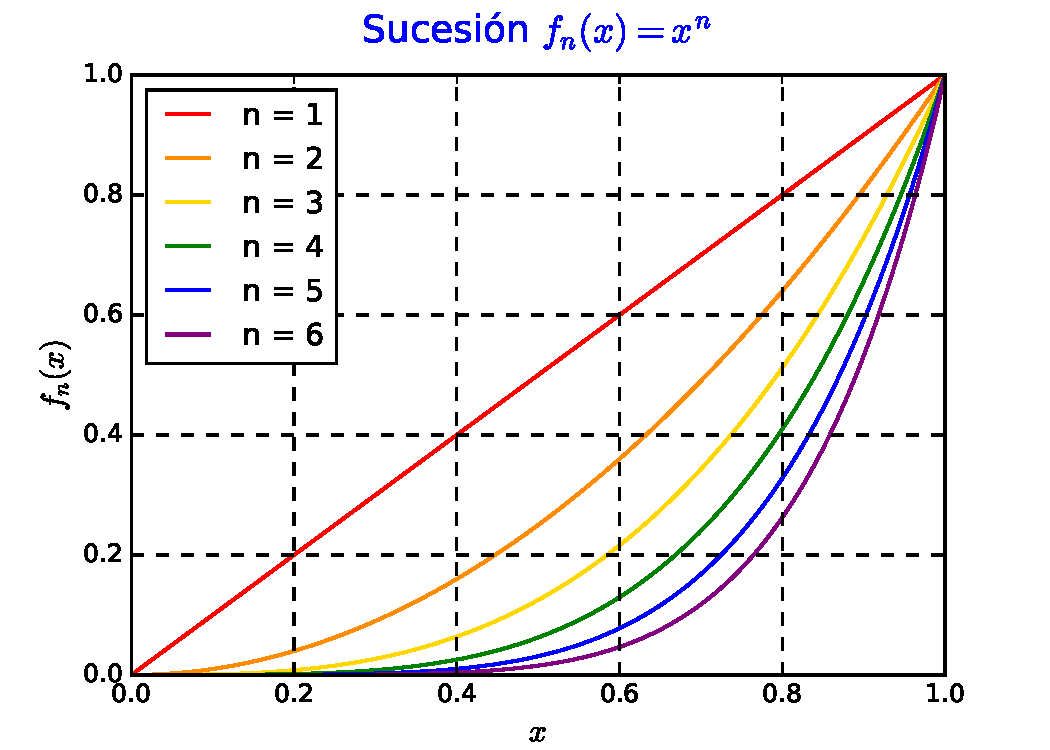
\includegraphics[scale=0.6]{Figuras/SucesionPolinomios.pdf}
\caption{Sucesión de polinomios $x^n, 0 \leq x \leq 1$ para $n = 1,2, \dots,6$.}
\end{center}
\end{figure}
\vspace{-0.7cm}

 y su función límite viene dada por
$$f(x) = \lim_{n\to + \infty} x^n = \left\{ \begin{array}{cl}
0,& 0 \leq x < 1 \\
1 ,& x = 1
\end{array} \right. .$$

Note que a pesar que cada término de la sucesión es continuo en $[0,1]$, $f$ no es continua en $x = 1$.
\end{ejemplo}

\begin{teorema}\label{UniformeContinuo}
Si $\{f_n\}_{n=1}^{\infty}$ es una sucesión de funciones complejas que converge uniformemente a $f$ en un dominio $D$ y cada función $f_n$ es continua en cada punto $z_0 \in D$, entonces la función límite $f$ también es continua en $z_0$.
\end{teorema}

\begin{proof}
Por convergencia uniforme, dado $\varepsilon > 0$, $\exists N \in \mathbb{N}$ tal que
$$n \geq N   ~\wedge~  z \in D ~\Rightarrow~ |f_n(z) - f(z)| < \frac{\varepsilon}{3}.$$

Además, por la continuidad de $f_N$ en $z_0$, existe $\delta = \delta (\varepsilon, N, z_0)$ tal que
$$\forall z: ~ 0 < |z-z_0| < \delta, z \in D ~\Rightarrow~ |f_N(z) - f_N(z_0)| < \frac{\varepsilon}{3}.$$

Por lo tanto,
\begin{align*}
\forall z:~ 0 < |z-z_0| < \delta, z \in D &\Rightarrow |f(z) - f(z_0)| \\
&= |f(z) - f_N(z) + f_N(z) - f_N(z_0) + f_N(z_0) - f(z_0)| \\
&\leq |f(z) - f_N(z)| + |f_N(z) - f_N(z_0)| + |f_N(z_0) - f(z_0)| \\
&< \frac{\varepsilon}{3} + \frac{\varepsilon}{3} + \frac{\varepsilon}{3} = \varepsilon.
\end{align*}
\end{proof}

A veces usamos el teorema \ref{UniformeContinuo} para probar que una sucesión no converge uniformemente.

\begin{ejemplo}
Una sucesión de funciones es definida en el disco unitario por \footnote{Para una visión gráfica puede acceder al siguiente archivo \href{https://www.geogebra.org/m/bedmcah3}{Geogebra}.}
$$f_n(z) =  \left\{ \begin{array}{cl}
n|z|,& \mbox{si}~~ |z| \leq \frac{1}{n} \\
1 ,& \mbox{si}~~  \frac{1}{n} < |z| \leq 1
\end{array} \right. .$$

¿La sucesión converge uniformemente para $|z| \leq 1$?
\\

\textbf{Solución:} Es claro que cada $f_n$ es continua en $\{z \in \mathbb{C} : |z| \leq 1\}$ y
$$\lim_{n \to + \infty} f_n(z) =  \left\{ \begin{array}{cl}
1,& \mbox{si}~~ 0 < |z| \leq 1 \\
0 ,& \mbox{si}~~  z = 0
\end{array} \right. .$$

Dado que la función límite no es continua en $z =0$, podemos concluir, a partir del teorema \ref{UniformeContinuo}, que $\{f_n\}_{n = 1}^{\infty}$ no converge uniformemente en cualquier conjunto que contenga al 0, en particular, no converge uniformemente para $|z| \leq 1$.
\end{ejemplo}

\begin{corolario}  \label{UniformeSerieContinuo}
Si una serie de funciones $\sum\limits_{n=1}^{\infty} f_n$ converge uniformemente a la función $f$ en un conjunto $D \subseteq \mathbb{C}$, y si cada término $f_n$ es continuo en un punto $z_0 \in D$, la suma $f$ también es continua en $z_0$. Simbólicamente este resultado se expresa como
$$\lim_{z\to z_0} \sum_{n=1}^{\infty} f_n(z) = \sum_{n=1}^{\infty} \lim_{z\to z_0} f_n(z).$$
\end{corolario}

\begin{proof}
Si cada término $f_n$ es una función continua en $z_0$, entonces cada suma parcial $s_n$ es continua en $z_0$. Luego, por el teorema \ref{UniformeContinuo}, la suma $f$ es continua en $z_0$.
\end{proof}

\begin{teorema}[Criterio de Cauchy*]
\ 

\begin{itemize}
    \item[(i)] Una sucesión $f_n(z)$ converge uniformemente en $D$ si y sólo si para cualquier $\varepsilon > 0$, existe $N \in \mathbb{N}$ tal que 
    $$n \geq N ~\wedge~  z \in D  \Rightarrow |f_n(z) - f_{n+p}(z)| < \varepsilon, \quad \mbox{para} ~ p = 1,2,3 \dots$$
    
    \item[(ii)] Una serie $\sum\limits_{n=1}^{\infty} f_n(z)$ converge uniformemente en $D$ si para todo $\varepsilon > 0$, existe $N \in \mathbb{N}$ tal que 
    $$n \geq N ~\wedge~ z \in D  \Rightarrow \left|\sum_{k=n+1}^{n+p} f_k(z)\right| < \varepsilon, \quad \mbox{para} ~ p = 1,2,3 \dots$$
\end{itemize}
\end{teorema}

\begin{proof}
Probaremos solo (i). 

Supongamos que $f_n \to f$ uniformemente en $D$, entonces dado $\varepsilon > 0$, $\exists N\in \mathbb{N} $ tal que
$$n \geq N ~\wedge~  z \in D ~\Rightarrow~ |f_n(z) - f(z)| < \frac{\varepsilon}{2}.$$

Como $n+p \geq N$, 
\begin{align*}
n \geq N ~\wedge~  z \in D &\Rightarrow |f_n(z) - f_{n+p}(z)| \\
&\leq |f_n(z) - f(z)| + |f(z) - f_{n+p}(z)| \\
&< \frac{\varepsilon}{2} + \frac{\varepsilon}{2} = \varepsilon, \quad p = 1,2,3, \dots
\end{align*}

Nos queda por probar la implicancia hacia la izquierda. Sea $f(z) = \lim\limits_{n\to + \infty} f_n(z)$, el cual existe porque para cada $z \in D$, $\{f_n(z)\}_{n=1}^{\infty}$ es una sucesión de Cauchy. Queremos mostrar que $f_n \to f$ uniformemente en $D$.

Dado $\varepsilon > 0$, podemos elegir un $N \in \mathbb{N}$ tal que 
$$n \geq N ~\wedge~  z \in D ~\Rightarrow~ |f_n(z) - f_{n+p}(z)| < \frac{\varepsilon}{2}, \quad p = 1,2,3, \dots$$

Como
$$\lim_{p \to + \infty} |f_n(z) - f_{n+p}(z)| = |f_n(z) - f(z)|,$$

existe $N_0 \in \mathbb{N}$ tal que
\begin{align*}
    \forall p: ~ p \geq N_0 &\Rightarrow  ||f_n(z) - f_{n+p}(z)| - |f_n(z) - f(z)|| < \frac{\varepsilon}{2} \\
    &\Rightarrow |f_n(z) - f(z)| - \frac{\varepsilon}{2} < |f_n(z) - f_{n+p}(z)| < |f_n(z) - f(z)| + \frac{\varepsilon}{2} \\
    & \Rightarrow |f_n(z) - f(z)| - \frac{\varepsilon}{2} < |f_n(z) - f_{n+p}(z)|.
\end{align*}

Luego,
\begin{align*}
n \geq N ~\wedge~  z \in D &\Rightarrow |f_n(z) - f(z)| - \frac{\varepsilon}{2} < |f_n(z) - f_{n+p}(z)| < \frac{\varepsilon}{2}, \quad p = N_0, N_0 +1,\dots \\
&\Rightarrow |f_n(z) - f(z)| - \frac{\varepsilon}{2} < \frac{\varepsilon}{2} \\
&\Rightarrow |f_n(z) - f(z)| < \varepsilon.
\end{align*}

Esto prueba que $f_n \to f$ uniformemente en $D$.

\end{proof}

Discutamos ahora un test de convergencia uniforme muy útil para series de funciones

\begin{teorema}[Criterio de M de Weierstrass] 
Sea $ \sum\limits_{n=1}^{\infty} f_n$ una sucesión de funciones complejas definidas en un dominio $D \subseteq \mathbb{C}$ y sea $\{M_n\}_{n=1}^{\infty}$ una sucesión de números reales tales que para todo $n \in \mathbb{N}$:
\begin{itemize}
    \item[(i)] $|f_n(z)| \leq M_n$ para todo $z \in D$, y
    
    \item[(ii)] $\sum\limits_{n=1}^{\infty} M_n $ converge.
\end{itemize}

 Entonces, la serie $\sum\limits_{n=1}^{\infty} f_n$ converge absolutamente y uniformemente en $D$.
 
\end{teorema}

\begin{proof}
Como la serie $\sum\limits_{n=1}^{\infty} M_n$ converge, usando el criterio de Cauchy para series reales, dado $\varepsilon > 0$, existe $N \in \mathbb{N}$ tal que
$$\forall n ,m \geq N, m > n ~\Rightarrow~ \left| \sum_{k=n+1}^m M_k  \right| =  \sum_{k=n+1}^m M_k < \varepsilon. $$

En particular, para $m = n + p$ con $p = 1,2, \dots$, tenemos que
$$\sum_{k=n+1}^{n + p} M_k < \varepsilon; \quad p = 1,2, \dots$$

Entonces,
$$  n \geq N ~\wedge~  z \in D \Rightarrow \left|\sum_{k = n+1}^{n+p} f_k(z) \right| 
\leq \sum_{k = n+1}^{n+p} |f_k(z)| 
 \leq  \sum_{k=n+1}^{n + p} M_k < \varepsilon; \quad p = 1,2, \dots
$$

y, por lo tanto, por el criterio de Cauchy, tenemos el resultado deseado.
\end{proof}

\begin{ejemplo}
Estudie la convergencia uniforme de 
$$f(z) = \sum_{n=1}^{\infty} \frac{\sin(nz)}{2^n}.$$

\textbf{Solución:} Notemos que
\begin{align*}
    \forall n \in \mathbb{N}: ~ \left|\frac{\sin(nz)}{2^n} \right| &= \frac{1}{2^n} \left| \frac{e^{inz} - e^{-inz}}{2i} \right| \\
    &= \frac{1}{2^{n+1}} \left| e^{-ny} e^{inx} - e^{ny} e^{-inx}\right|, \quad (z = x+iy) \\
    &\leq \frac{1}{2^{n+1}} \left[ |e^{-ny}| \,|e^{inx}| + |e^{ny}| \,|e^{-inx}| \right] \\
    &= \frac{1}{2^{n+1}} \left[ \frac{1}{e^{ny}} + e^{ny} \right] \\
    &= \frac{1}{2} \left[ \left( \frac{1}{2e^{y}}\right)^n +  \left( \frac{e^y}{2}\right)^n \right] = M_n.
\end{align*}

La serie $\sum\limits_{n=1}^{\infty} M_n$ converge si y sólo si
$$\left|\frac{1}{2e^y}\right| < 1 ~\wedge~ \left|\frac{e^y}{2}\right|<1  \Leftrightarrow \frac{1}{2} < e^y < 2 \Leftrightarrow - \ln(2) < y < \ln(2) \Leftrightarrow |y| < \ln(2).$$

Por el criterio de M de Weierstrass, $f(z)$ converge absolutamente y uniformemente en $\{z \in \mathbb{C} : |Im(z)| < \ln(2)\}$.
\end{ejemplo}

\subsection*{Integración y analiticidad de sucesiones y series de funciones}

\begin{teorema} \label{IntegracionUniforme}
Sea $\gamma$ una curva suave a trazos en una región $D$ y sea $\{f_n\}_{n=1}^{\infty}$ una sucesión de funciones complejas continuas, las cuales convergen uniformemente a $f$ en $\gamma$. Entonces,
$$\lim_{n\to + \infty} \int_{\gamma} f_n(z) \,dz = \int_{\gamma} f(z) \,dz.$$
\end{teorema}

\begin{proof}
La función $f$ es continua, por el teorema \ref{UniformeContinuo} y, por tanto, es integrable. Por hipótesis, para $\varepsilon > 0$ dado, existe $N \in \mathbb{N}$ tal que
$$n \geq N \Rightarrow \left| f_n(z) - f(z)\right| < \frac{\varepsilon}{l(\gamma)};\quad \forall z \in \gamma.$$

Integrando la última expresión, tenemos 
$$\left| \int_{\gamma} f_n(z) \,dz - \int_{\gamma} f(z) \, dz\right| = \left| \int_{\gamma} [f_n(z) - f(z)] \,dz\right| \leq \int_{\gamma} |f_n(z) - f(z)| \,|dz| < \frac{\varepsilon}{l(\gamma)} l(\gamma) =\varepsilon,$$

a partir de la cual se demuestra lo requerido.
\end{proof}

\begin{corolario} \label{IntegracionSerieUniforme}
Sea $\gamma$ una curva suave a trazos en una región $D$ y sea $\{f_n\}_{n=1}^{\infty}$ una sucesión de funciones complejas continuas. Si  $\sum\limits_{n=1}^{\infty} f_n$ converge uniformemente en $\gamma$, entonces $\sum\limits_{n=1}^{\infty} f_n$ es integrable en $\gamma$ y 
$$\int_{\gamma} \left( \sum_{n=1}^{\infty} f_n(z)\right)\, dz = \sum_{n=1}^{\infty} \int_{\gamma} f_n(z) \, dz.$$
\end{corolario}

\begin{proof}
Se aplica el teorema \ref{IntegracionUniforme} a la sucesión de sumas parciales $\{s_n\}_{n=1}^{\infty}$ dada por
$$s_n(z) = \sum_{k=1}^n f_n(z)$$

y observamos que 
$$\int_{\gamma} s_n(z) \, dz = \sum_{k=1}^n \int_{\gamma} f_n(z) \,dz.$$

\end{proof}

\begin{teorema} \label{DerivadasUniforme}
Supongamos que $\{f_n\}_{n=1}^{\infty}$ es una sucesión de funciones complejas analíticas en una región $D$ tal que converge uniformemente a $f$ en cualquier disco cerrado contenido en $D$. Entonces,
\begin{itemize}
    \item[(i)] $f$ es analítica en $D$, y
    
    \item[(ii)] para todo $k \in \mathbb{N}$, 
    $$\lim_{n\to + \infty}\frac{d^k}{d z^k} f_n(z) = \frac{d^k}{dz^k}f(z), \quad \forall z \in D.$$
    
    Además, la convergencia de sus derivadas es uniforme en cualquier disco cerrado en $D$.
\end{itemize}
\end{teorema}

\begin{proof}
\ 

\begin{itemize}
    \item[(i)] Sea $z_0 \in D$, como $D$ es abierto, existe un disco abierto $B(z_0,R) \subseteq D$. Si consideramos $0 < r < R$, $\overline{B}(z_0,r)$ es un disco cerrado contenido en $D$. Como $\{f_n\}_{n=1}^{\infty}$ converge uniformemente en $\overline{B}(z_0,r)$ es claro que también lo hace en el disco abierto $B(z_0,r)$. Queremos mostrar que $f$ es analítica en $B(z_0,r)$. Por el teorema \ref{UniformeContinuo}, $f$ es continua en $B(z_0,r)$. Ahora, para  cualquier curva cerrada $\gamma$ contenida en $B(z_0,r)$, el teorema de Cauchy nos dice que
    $$\int_{\gamma} f_n(z) \,dz = 0.$$
    
  Por el teorema \ref{IntegracionUniforme}, tenemos que $$\int_{\gamma} f(z) \,dz = \lim_{n\to + \infty} \int_{\gamma} f_n(z) \,dz = 0.$$
    
    Entonces, por el teorema de Morera, $f$ es analítica en $B(z_0,r)$ y como $z_0$ es arbitrario, $f$ es analítica en todo $D$.
    
    \item[(ii)] Basta probar que 
    \begin{equation}
      \forall z \in D:~ \lim_{n \to + \infty} f'_n(z) = f'(z),  \label{DerivadaUniforme0}
    \end{equation}

    donde la derivada converge uniformemente en todo disco cerrado. Para ello, sean $z_0 \in D$ y $R > 0$ tal que el disco $\overline{B}(z_0,r) \subset B(z_0,R) \subset D$. Consideremos la circunferencia $C_R: |z-z_0| = R$, por la fórmula de la integral de Cauchy,
    \begin{equation}
      f'_n(z) = \frac{1}{2\pi i} \int_{C_R} \frac{f_n(\xi)}{(\xi-z)^2} \,d\xi ~~\mbox{y}~~ f'(z) = \frac{1}{2\pi i} \int_{C_R}\frac{f(\xi)}{(\xi-z)^2} \,d\xi, \quad z \in \overline{B}(z_0,r). \label{DerivadaUniforme1}
    \end{equation}
    
    Por otro lado, de la convergencia uniforme, tenemos que para un $\varepsilon > 0$ dado, existe $N \in \mathbb{N}$ tal que
    \begin{equation}
       n \geq N ~\wedge~  z \in \Tilde{D} \Rightarrow |f_n(z) - f(z)| < \varepsilon, \label{DerivadaUniforme2}
    \end{equation}
    
    donde $\Tilde{D}$ es cualquier disco cerrado contenido en $D$.
    
    De esta manera, si combinamos \eqref{DerivadaUniforme1} y \eqref{DerivadaUniforme2}, concluimos que
    \begin{align*}
       n \geq N ~\wedge~  z \in \overline{B}(z_0,r) \Rightarrow \left|f_n'(z) - f'(z) \right| &= \left|\frac{1}{2\pi i} \int_{C_R} \frac{f_n(\xi) - f(\xi)}{(\xi-z)^2}\,d\xi \right| \\
        &\leq \frac{1}{2\pi} \int_{C_R}  \frac{|f_n(\xi) - f(\xi)|}{|\xi-z|^2}\,|d\xi|\\
        & < \frac{1}{2\pi} \int_{C_R}  \frac{\varepsilon}{|\xi-z|^2}\,|d\xi| \\
        &\leq \frac{\varepsilon}{2\pi} \frac{l(C_R)}{(R-r)^2} = \frac{\varepsilon R}{(R-r)^2},
    \end{align*}
    
pues $|\xi - z| > R-r$.

Como $z_0$ es arbitrario, hemos probado la convergencia uniforme en todo disco cerrado contenido en $D$ y la validez de \eqref{DerivadaUniforme0}.
\end{itemize}
\end{proof}

\begin{corolario}
 Si $\{f_n\}_{n=1}^{\infty}$es  una sucesión de funciones complejas analíticas en una región $D$ y   $\sum\limits_{n=1}^{\infty} f_n$ converge uniformemente en cualquier disco cerrado en $D$, entonces
 \begin{itemize}
    \item[(i)] $\sum\limits_{n=1}^{\infty} f_n = S$ es analítica en $D$, y
    
    \item[(ii)] para todo $k \in \mathbb{N}$, 
    $$ \frac{d^k}{dz^k}S(z) = \sum_{n=1}^{\infty} \frac{d^k}{dz^k} f_n(z), \quad \forall z \in D.$$
    
    Además, la convergencia de sus derivadas es uniforme en cualquier disco cerrado en $D$.
\end{itemize}
\end{corolario}

\begin{proof}
Aplicar el teorema \ref{DerivadasUniforme} a la sucesión de sumas parciales $s_n = f_1 + f_2 + \cdots + f_n$.
\end{proof}

\textbf{Observación:} El teorema \ref{DerivadasUniforme} y su corolario se conocen a veces por el teorema de Weierstrass.

Por otro lado, éstos revelan otra remarcable propiedad de las funciones analíticas, que no es compartida por las funciones de variable real. La convergencia uniforme usualmente no es suficiente para justificar la diferenciación de una serie término a término, pero para las funciones analíticas, ésto es suficiente.


\begin{ejemplo}[Certamen 2 (2020)]
Considere la función
$$f(z) = \sum_{n=0}^{\infty} \frac{1}{n! z^n}.$$

\begin{itemize}
    \item[(a)] Haga ver que $f$ es analítica en $\mathbb{C} \setminus \{0\}$.
    
    \item[(b)] Calcule
    $$\int_{\gamma} f(z) \,dz$$
    
    donde $\gamma$ es la circunferencia unitaria, orientada positivamente y de índice 1.
\end{itemize}

\textbf{Solución:}


\begin{itemize}
    \item[(a)] Sea $\varepsilon > 0$ cualquiera tal que $|z| > \varepsilon$. Notemos que para cada $n\in \mathbb{N}_0$:
    $$\left| \frac{1}{n! z^n} \right| = \frac{1}{n! |z|^n} < \frac{1}{n! \varepsilon^n} = M_n.$$
    
    Analicemos la convergencia de $\sum\limits_{n=0}^{\infty}M_n $, para ello calculemos
    $$\lim_{n\to + \infty} \left| \frac{M_{n+1}}{M_n}\right| = \lim_{n\to + \infty} \frac{n! \varepsilon^n}{(n+1)! \varepsilon^{n+1}} = \frac{1}{\varepsilon} \lim_{n\to + \infty} \frac{1}{n+1} = 0 = L.$$
    
    Como $L = 0 < 1$, el criterio del cociente nos dice que $\sum\limits_{n=0}^{\infty}M_n $ converge.
    
    Usando el criterio de M de Weierstrass, la serie $\sum\limits_{n=0}^{\infty} \frac{1}{n! z^n}$ converge absolutamente y uniformemente en $\{z \in \mathbb{C}: |z|> \varepsilon\}$, pero $\varepsilon$ es arbitrario. Por lo tanto, la serie converge uniformemente en $\mathbb{C} \setminus \{0\}$.
    
    Ahora cada función $\frac{1}{n! z^n}$ es analítica en $\mathbb{C} \setminus \{0\}$ y la serie $\sum\limits_{n=0}^{\infty} \frac{1}{n! z^n}$ converge uniformemente en todo disco cerrado en  $\mathbb{C} \setminus \{0\}$. Entonces, por el teorema de Weierstrass, $f(z)$ es analítica en $\mathbb{C} \setminus \{0\}$.
    
    \item[(b)] La curva $\gamma$ es suave, cerrada y simple (índice igual a 1), la serie $\sum\limits_{n=0}^{\infty} \frac{1}{n! z^n}$ es uniformemente convergente en $\mathbb{C} \setminus \{0\}$, más aún en $\gamma$ y cada $\frac{1}{n! z^n}$ es continua en $\gamma$. Entonces, por el teorema \ref{IntegracionSerieUniforme}, se tiene que
    $$\int_{\gamma} \left(\sum_{n=0}^{\infty} \frac{1}{n! z^n} \right) \,dz = \sum_{n=0}^{\infty} \int_{\gamma} \frac{1}{n! z^n} \,dz.$$
    
    Para $n = 0$:
    $$\int_{\gamma}  \frac{1}{n! z^n} \,dz = \int_{\gamma} 1 \,dz = 0,$$
    
    por el teorema de Cauchy-Goursat, ya que $g(z) = 1$ es entera.
    
    Para $n = 1$:
    $$\int_{\gamma} \frac{1}{n! z^n} \,dz = \int_{\gamma} \frac{1}{z} \,dz.$$
    
    Como $g(z) = 1$ es entera, el teorema de la fórmula integral de Cauchy nos dice que
    $$\int_{\gamma} \frac{1}{z} \,dz = 2\pi i.$$
    
    Para $n\geq 2$, la función $h(z) = \frac{1}{n!}$ es entera, entonces, por el teorema de la fórmula integral de Cauchy, tenemos que
    $$\int_{\gamma} \frac{h(z)}{z^n} \,dz = \frac{2\pi i}{(n-1)!} h^{(n-1)}(0) = 0.$$
    
    Por lo tanto,
    $$\int_{\gamma} f(z) \,dz = 2\pi i.$$
\end{itemize}
\end{ejemplo}

\section{Series de potencias}

\begin{defi}
Una \textbf{serie de potencias} es una serie de funciones de la forma
$$\sum_{n=0}^{\infty} a_n(z-z_0^n) = a_0 + a_1 (z-z_0) + \cdots + a_n (z-z_0)^n + \cdots$$

donde $\{a_n\}_{n=1}^{\infty}$ es una sucesión de números complejos, $z \in \mathbb{C}$ una variable y $z_0 \in \mathbb{C}$ fijo es el \textbf{centro} de la serie de potencias.
\end{defi}

\textbf{Observación:} Note que en la definición se usó la convención $(z-z_0)^{0} = 1$ para todo $z \in \mathbb{C}$. Una serie de potencias siempre converge en su centro $z = z_0$ al valor $a_0$. Para $z \neq z_0$ la serie de potencias puede converger o diverger.

\begin{ejemplo}
Estudie la convergencia de la serie de potencias
$$\sum_{n=0}^{\infty} (-2)^n \frac{z^n}{n+1}.$$

\textbf{Solución:} Para $z = 0$, la serie converge a $2$. 

Para $z \neq 0$, usemos el criterio del cociente:
$$\lim_{n\to + \infty} \left| \frac{(-2)^{n+1} z^{n+1}(n+1)}{(-2)^n z^n (n+2)}  \right| = \lim_{n\to + \infty} 2|z| \frac{n+1}{n+2} = 2|z|.$$

Entonces, la serie converge si $2|z| < 1$ y diverge si $2|z| >1 $. Equivalentemente, la serie converge si $|z| < \frac{1}{2}$ y diverge si $|z| > \frac{1}{2}$.
\end{ejemplo}

\textbf{Observación:} Haciendo el cambio de variable $w = z-z_0$ en la serie de potencias \newline $\sum\limits_{n=0}^{\infty} a_n(z-z_0)^n$, se transforma en $\sum\limits_{n=0}^{\infty} a_n w^n$. En consecuencia, para estudiar las propiedades de $\sum\limits_{n=0}^{\infty} a_n(z-z_0)^n$ basta estudiar la serie de potencias $\sum\limits_{n=0}^{\infty} a_n w^n$.

\begin{teorema}\label{ConvergenciaPotencia}
Si la serie de potencias $\sum\limits_{n=0}^{\infty} a_nz^n$ converge en un punto $z = z_1 \neq 0$, se tiene:

\begin{itemize}
\item[(a)] La serie converge absolutamente para todo $z$ siendo $|z| < |z_1|$.

\item[(b)] La serie converge uniformemente en $|z| \leq R$ con $R < |z_1|$.
\end{itemize}
\end{teorema}

\begin{proof}
Notemos que
\begin{equation}
\forall z \in \overline{B}(0,R):~ |a_n z^n| = |a_n| |z_1|^n \left(\left| \frac{z}{z_1} \right| \right)^n \leq |a_n| |z_1|^n \left(\left| \frac{R}{z_1} \right|  \right)^n \label{Potencia1}
\end{equation}

Como $\sum\limits_{n=0}^{\infty} a_n z_1^n$ converge, $\lim\limits_{n \to + \infty} a_nz_1^n = 0$, por consiguiente existe $M > 0$ tal que
$$\forall n \geq 0:~ |a_n z_1^n| \leq M.$$

Así, la expresión \eqref{Potencia1} nos queda
\begin{equation}
\forall z \in \overline{B}(0,R) :~ |a_n z^n| \leq M\left(\left| \frac{R}{z_1} \right|  \right)^n \label{Potencia2}
\end{equation}

Dado que $R < |z_1| ~\Rightarrow~ \left| \frac{R}{z_1} \right| <1$, la serie geométrica $\sum\limits_{n=0}^{\infty} \left| \frac{R}{z_1} \right|^n$ converge.

Luego, por el criterio M de Weierstrass, la serie $\sum\limits_{n=0}^{\infty} a_n z^n$ converge uniformemente en $|z| \leq R$. Ésto prueba \textit{(b)}.

Usando \eqref{Potencia2} y el criterio de comparación directa, la serie $\sum\limits_{n=0}^{\infty} a_n z^n$ converge absolutamente para $|z| \leq R < |z_1|$.

\end{proof}

\textbf{Observación:} Del teorema, si $\sum\limits_{n=0}^{\infty} a_n z_1^n$ diverge, entonces también diverge la serie $\sum\limits_{n=0}^{\infty} a_n z^n$ para $|z| > |z_1|$.
\\

Definamos 
$$R := \sup \left\{|z| : \sum_{n=0}^{\infty} a_n z^n < \infty  \right\}.$$

Este valor es finito si existe algún $z$ para el cual la serie $\sum\limits_{n=0}^{\infty} a_n z^n$ converge  y vale $+\infty$ en otro caso.

\begin{defi}
Al valor $R$ lo llamaremos el \textbf{radio de convergencia} de la serie de potencias $\sum\limits_{n=0}^{\infty} a_n z^n$ .
\end{defi}

\begin{defi}
El conjunto $D$ de todos los $z$ complejos para los cuales la serie $\sum\limits_{n=0}^{\infty} a_n z^n$ converge se llama \textbf{región de convergencia}. 
\end{defi}

\textbf{Observación:} Notemos que $B(0,R) \subseteq D \subseteq \overline{B}(0,R)$.

\begin{teorema}[Existencia de la región de convergencia]
Si la serie de potencias $\sum\limits_{n=0}^{\infty} a_n z^n$ converge por lo menos para un $z = z_1 \neq 0$, y diverge por lo menos para $z = z_2$, existe un número real positivo $R$ tal que la serie converge absolutamente si $|z| < R$ y diverge si $|z| > R$.
\end{teorema}

\begin{proof}
Sea 
$$I = \left\{ |z| : \sum_{n=0}^{\infty} a_n z^n < + \infty  \right\}.$$

El conjunto $I \neq \emptyset$, ya que por hipótesis contiene a $|z_1|$. Asimismo, ningún número de $I$ puede ser mayor que $|z_2|$, debido al teorema \ref{ConvergenciaPotencia}.

Luego, $|z_2|$ es cota superior de $I$ y, por el axioma del supremo, existe
$$R = \sup I > 0.$$

En virtud del teorema \ref{ConvergenciaPotencia}, ningún número de $I$ puede superar a $R$. Por consiguiente, la serie diverge si $|x| > R$.

Para demostrar que la serie converge absolutamente si $|z| < R$, debemos notar que existe $|\Tilde{z}|$ en $I$ tal que $|z| < |\Tilde{z}| < R$ y por el teorema \ref{ConvergenciaPotencia}, la serie converge absolutamente.

\end{proof}

Para el caso de serie de potencias centradas en $z_0 \neq 0$, basta hacer el estudio haciendo la sustitución $w = z-z_0$.

Luego, dada la serie $\sum\limits_{n=0}^{\infty} a_n(z-z_0)^n$, se verifica una de las siguiente tres posibilidades:
\begin{enumerate}
\item La serie converge sólo para $z_0$.

\item Existe $R > 0$ tal que la serie converge para $|z-z_0| < R$ y diverge para $|z-z_0| > R$.

\item La serie converge para todo $z \in \mathbb{C}$.
\end{enumerate}

\textbf{Observación 1:} En el caso 1., $R = 0$ y en el caso 3., $R =  + \infty$.

\textbf{Observación 2:} $|z-z_0| = R$ es el \textbf{círculo de convergencia} y, en general, no está garantizada la convergencia de la serie en él.

\begin{figure}[H]
    \centering
    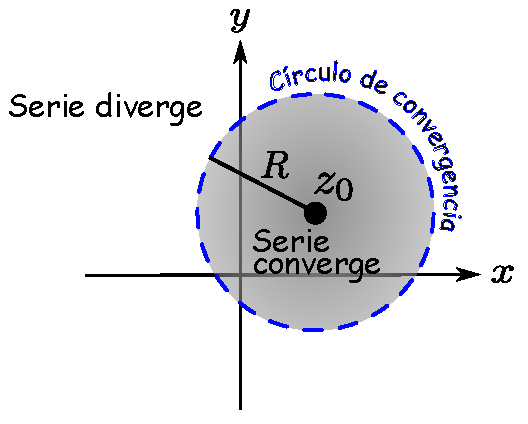
\includegraphics[scale = 0.8]{Figuras/ConvergenciaSeriePotencia.pdf}
    \caption{Región de convergencia de una serie de potencia.}
    \label{fig:CVPotencia}
\end{figure}

\subsection*{Continuidad, integración y analiticidad de las series de potencias}

Aplicando los teoremas vistos para el tratamiento de sucesiones y series de funciones, tenemos:

\begin{propo}
La suma de una serie de potencias es continua en la región de convergencia.
\end{propo}

\begin{propo}\label{IntegracionPotencia}
Si $\sum\limits_{n=0}^{\infty} a_n (z-z_0)^n$ es una serie de potencias y $\gamma$ una curva suave por trazos contenida en el interior de su círculo de convergencia, entonces
$$\int_{\gamma} \left( \sum_{n=0}^{\infty} a_n (z-z_0)^n \right) \,dz = \sum_{n=0}^{\infty} a_n \int_{\gamma} (z-z_0)^n \,dz.$$
\end{propo}

\begin{propo}\label{DerivadaPotencia}
Si $\sum\limits_{n=0}^{\infty} a_n (z-z_0)^n$ es una serie de potencias y $S(z)$ su suma, entonces $S(z)$ es derivable en cada punto $z$ al interior de su círculo de convergencia y su derivada puede obtenerse derivando término a término la serie $\sum\limits_{n=0}^{\infty} a_n (z-z_0)^n$, es decir,
$$S\,'(z) = \sum_{n=1}^{\infty} n a_n (z-z_0)^{n-1}.$$
\end{propo}

\begin{ejemplo}
Empecemos con la serie geométrica
$$\frac{1}{1 - z} = \sum_{n=0}^{\infty} z^n, \quad |z| < 1.$$

Hacemos el reemplazo $\xi = - z$ para asi obtener
$$\frac{1}{1 + \xi} = \sum_{n=0}^{\infty} (-1)^n \xi^n, \quad |\xi| < 1.$$

Como la integral de una función analítica en una bola abierta (simplemente conexo) es independiente de la curva, integramos en el segmento $[0,z]$, donde $|z| < 1$, 
$$\int_{[0,z]} \frac{1}{1+\xi} d\xi = \sum_{n=0}^{\infty} (-1)^n \int_{[0,1]} \xi^n \,d\xi.$$

Una antiderivada de la función continua $1/(1+\xi)$ en $\mathbb{C} - \{-1\}$ es $Log(1 + z)$ en la región $D = \mathbb{C}\setminus ]-\infty,-1]$. Entonces,
\begin{align*}
    Log(1+z) = \int_{[0,z]} \frac{1}{1+\xi} d\xi &= \sum_{n=0}^{\infty} \left. (-1)^n \frac{\xi^{n+1}}{n+1} \right|_{0}^z \\
    &= \sum_{n=0}^{\infty} (-1)^n \frac{z^{n+1}}{n+1}.
\end{align*}

Por lo tanto,
$$Log(1+z) = \sum_{n=0}^{\infty} (-1)^n \frac{z^{n+1}}{n+1}, \quad |z| < 1.$$
\end{ejemplo}

\begin{ejemplo}
Encuentre la suma de $\sum\limits_{n=1}^{\infty} n z^n$ y determine su radio de convergencia.
\\

\textbf{Solución:} Esta serie se ve como la derivada de la serie geométrica
$$\frac{1}{1-z} = \sum_{n=0}^{\infty} z^n, \quad |z| < 1.$$

En efecto, derivando término a término, obtenemos la serie de potencias
$$\frac{d}{dz}\left[ \frac{1}{1-z} \right] = \frac{1}{(1-z)^2} = \sum_{n=1}^{\infty} n z^{n-1}, \quad |z| < 1.$$

Multiplicando ambos lados por $z$, 
$$\frac{z}{(1-z)^2} = \sum_{n=1}^{\infty} n z^n, \quad |z| < 1.$$

En particular, el radio de convergencia es 1.
\end{ejemplo}

\begin{teorema}[Unicidad de la serie de potencias] 
Sea $R > 0$. Si para todo $z$ que satisface $|z-z_0| < R$, tenemos
$$\sum_{n=0}^{\infty} a_n (z-z_0)^n = f(z) =  \sum_{n=0}^{\infty} b_n(z-z_0)^n.$$

Entonces, $a_n = b_n$ para todo $n \in \mathbb{N}_0$. En particular, si $\sum\limits_{n=0}^{\infty} c_n (z-z_0)^n = 0$ para todo $|z-z_0| < R$, entonces $c_n = 0$ para $n = 0,1,2, \dots$
\end{teorema}

\begin{proof}
La proposición \ref{DerivadaPotencia} nos garantiza la existencia de las derivadas de orden superior para la misma región de convergencia de una serie de potencias. Entonces,
\begin{align*}
f'(z) &= \sum_{n=1}^{\infty} n a_n(z-z_0)^{n-1} = \sum_{n=1}^{\infty} n b_n(z-z_0)^{n-1} \\
f''(z) &= \sum_{n=2}^{\infty} n(n-1) a_n(z-z_0)^{n-2} = \sum_{n=2}^{\infty} n(n-1) b_n(z-z_0)^{n-2} \\
&~\vdots \\
f^{(k)} (z) &=  \sum_{n=k}^{\infty} n(n-1) \cdots (n-(k-1)) a_n(z-z_0)^{n-k} = \sum_{n=k}^{\infty} n(n-1) \cdots (n - (k-1)) b_n(z-z_0)^{n-k}.
\end{align*}

Evaluando en $z = z_0$ y considerando $f^{(0)}(z_0) = f(z_0)$:
$$\forall k \geq 0: ~ f^{(k)}(z_0) = k! a_k = k! b_k ~\Rightarrow~ a_k = b_k.$$
\end{proof}

\section{Series de Taylor}

Sea $f$ una función analítica en un dominio $D$ y sea $z_0 \in D$. Por el teorema de la fórmula integral de Cauchy, $f$ tiene derivada de todos los órdenes en $z_0$.

\begin{defi}
Se define la serie de potencias siguiente:
$$f(z_0) + \sum_{n=1}^{\infty} \frac{f^{(n)}(z_0)}{n!}(z-z_0)^n.$$

Esta serie se llama \textbf{serie de Taylor} de $f$ alrededor de $z_0$.
\end{defi}

\textbf{Observación:} Cuando $z_0 = 0$, la serie se conoce como \textbf{serie de Maclaurin} de $f$.

\begin{teorema}[de Taylor]
Sea $f$ una función analítica en un dominio $D$ y sea $z_0 \in D$. Entonces, existe $R_0 > 0$ tal que la serie de Taylor de $f$ en $z_0$
$$f(z_0) + \sum_{n=1}^{\infty} \frac{f^{(n)}(z_0)}{n!}(z-z_0)^n.$$

converge para $|z-z_0| < R_0$; más aún, su suma es $f(z)$, es decir,
$$f(z) = f(z_0) + \sum_{n=1}^{\infty} \frac{f^{(n)}(z_0)}{n!}(z-z_0)^n.$$
\end{teorema}

\begin{proof}

Dado que $D$ es abierto, elegimos el mayor $R_0 > 0$ tal que $B(z_0,R_0) \subseteq D$, es decir, el mayor disco abierto tal que $f$ sea analítica. Para $0 < R_1 < R_0$, tomamos $z$ al interior de la circunferencia $C_1: |z-z_0| = R_1$, ver figura \ref{fig:Taylor}. Como $f$ es analítica, por el teorema de la fórmula integral de Cauchy, 
$$f(z) = \frac{1}{2\pi i} \int_{C_1} \frac{f(\xi)}{\xi-z} d\xi.$$

\begin{figure}[H]
    \centering
    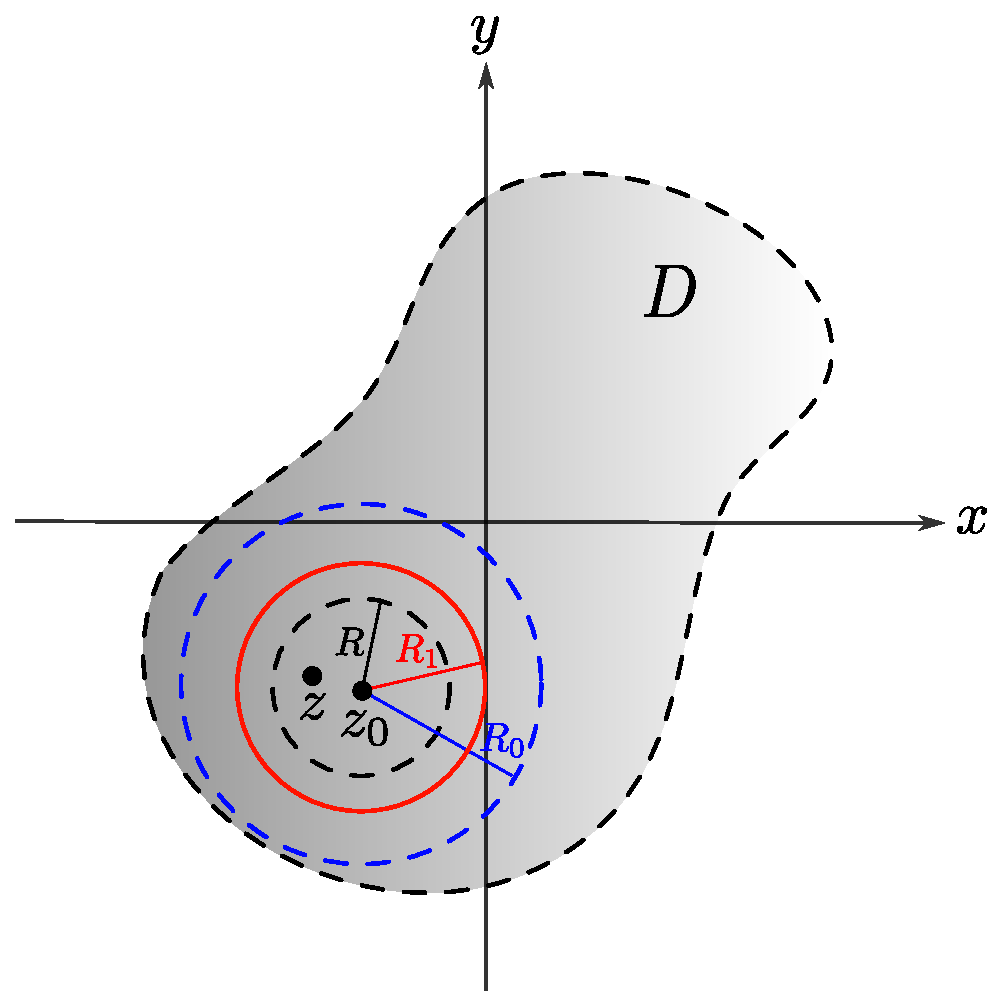
\includegraphics[scale = 0.55]{Figuras/TeoremaTaylor.pdf}
    \caption{Demostración del teorema de Taylor.}
    \label{fig:Taylor}
\end{figure}

Sea $\xi \in C_1$, notemos que
$$\frac{1}{\xi - z} = \frac{1}{(\xi - z_0) - (z-z_0)} = \frac{1}{\xi - z_0} \frac{1}{1- \frac{z-z_0}{\xi-z_0}}. $$

Del ejemplo \ref{SerieGeo}, se tiene que
$$\sum_{k=0}^n w^k = 1 + w + \cdots + w^n = \frac{1-w^{n+1}}{1-w}, \quad w \neq 1.$$

Entonces,
\begin{align*}
    \frac{1-\left(\frac{z-z_0}{\xi-z_0}\right)^N}{1- \frac{z-z_0}{\xi-z_0}} &= 1 + \frac{z-z_0}{\xi-z_0} + \left(\frac{z-z_0}{\xi-z_0} \right)^2 + \cdots + \left(\frac{z-z_0}{\xi-z_0} \right)^{N-1} \\
    \Rightarrow ~ \frac{1}{1- \frac{z-z_0}{\xi-z_0}}&=  1 + \frac{z-z_0}{\xi-z_0} + \left(\frac{z-z_0}{\xi-z_0} \right)^2 + \cdots + \left(\frac{z-z_0}{\xi-z_0} \right)^{N-1} + \frac{1}{1-\frac{z-z_0}{\xi-z_0}} \left(\frac{z-z_0}{\xi-z_0} \right)^{N}.
\end{align*}

Así,
\begin{align*}
    \frac{1}{\xi-z} &= \frac{1}{\xi-z_0}  \frac{1}{1- \frac{z-z_0}{\xi-z_0}} \\
    &= \frac{1}{\xi-z_0} \left(  1 + \frac{z-z_0}{\xi-z_0} + \left(\frac{z-z_0}{\xi-z_0} \right)^2 + \cdots + \left(\frac{z-z_0}{\xi-z_0} \right)^{N-1} + \frac{1}{1-\frac{z-z_0}{\xi-z_0}} \left(\frac{z-z_0}{\xi-z_0} \right)^{N}\right) \\
    &= \frac{1}{\xi-z_0} + \frac{z-z_0}{(\xi-z_0)^2} + \cdots + \frac{(z-z_0)^{N-1}}{(\xi - z_0)^N} + \frac{(z-z_0)^N}{(\xi-z)(\xi - z_0)^N}.
\end{align*}

Luego,
\begin{align*}
    \frac{f(\xi)}{\xi-z} &= \frac{f(\xi)}{\xi-z_0} +(z-z_0) \frac{f(\xi)}{(\xi-z_0)^2} + (z-z_0)^2 \frac{f(\xi)}{(\xi-z_0)^3} + \cdots \\ & ~ + (z-z_0)^{N-1}\frac{f(\xi)}{(\xi - z_0)^N} +(z-z_0)^N \frac{f(\xi)}{(\xi-z)(\xi - z_0)^N}.
\end{align*}

Ahora, integrando ambos lados por $\frac{1}{2\pi i} \int_{C_1}$, tenemos
\begin{align*}
    f(z) &= \frac{1}{2\pi i} \int_{C_1} \frac{f(\xi)}{\xi-z} \,d\xi \\
    &= \frac{1}{2\pi i} \int_{C_1} \frac{f(\xi)}{\xi-z_0} \,d\xi + (z-z_0) \frac{1}{2\pi i} \int_{C_1} \frac{f(\xi)}{(\xi-z)^2} \,d\xi + (z-z_0)^2 \frac{1}{2\pi i} \int_{C_1} \frac{f(\xi)}{(\xi-z_0)^3} \,d\xi + \cdots \\
    &~+ (z-z_0)^{N-1} \frac{1}{2\pi i} \int_{C_1} \frac{f(\xi)}{(\xi-z_0)^N} \,d\xi + (z-z_0)^N \frac{1}{2\pi i} \int_{C_1} \frac{f(\xi)}{(\xi - z)(\xi - z_0)^N} \,d\xi \\
    &= f(z_0) + f'(z_0) (z-z_0) + \frac{f''(z_0)}{2!}(z-z_0)^2 + \frac{f^{(3)}(z_0)}{3!} (z-z_0)^3 + \cdots \\
    & ~+ \frac{f^{(N-1)}(z_0)}{(N-1)!} (z-z_0)^{N-1} + R_N(z), 
\end{align*}

donde 
$$R_N(z) =  \frac{(z-z_0)^N}{2\pi i} \int_{C_1} \frac{f(\xi)}{(\xi - z)(\xi - z_0)^N} \,d\xi.$$

Recordemos que $ |z-z_0| < R < R_1$ y $|\xi-z_0| = R_1$, de donde se obtiene
$$|\xi-z| \geq ||\xi - z_0| - |z-z_0|| \geq |\xi-z_0| - |z-z_0| > R_1 - R.$$

Luego, si $|f(\xi)| \leq M$ para $\xi \in C_1$ (compacto), entonces
$$|R_N(z)| \leq \frac{R^N}{2\pi} \frac{2\pi R_1 M}{(R_1 - R)R_1^N} = \frac{MR_1}{R_1- R} \left( \frac{R}{R_1}\right)^{N}.$$

Como $0 < \frac{R}{R_1} < 1$, se tiene que
$$\lim_{N \to + \infty} R_N(z) = 0,$$

probando así el teorema.
\end{proof}

\begin{ejemplo}
Encuentre las series de Maclaurin de 
$$(a) ~e^z, \quad (b)~ \cos z, \quad (c) ~\sin z. $$

\textbf{Solución:} Notemos que las tres funciones son enteras, así que las series de Maclaurin convergerán para todo $z \in \mathbb{C}$.

\begin{itemize}
    \item[(a)] Si $f(z) = e^z$, entonces
    $$\forall n \in \mathbb{N}: ~ f^{(n)}(z) = e^z \Rightarrow f^{(n)}(0) = 1.$$
    
    Por lo tanto, la serie de Macluarin es
    $$e^z = \sum_{n=0}^{\infty} \frac{f^{(n)}(0)}{n!} z^n = \sum_{n=0}^{\infty} \frac{z^n}{n!}, \quad \forall z \in \mathbb{C}.$$
    
    \item[(b)] Notemos que 
    \begin{align*}
f(z) = \cos(z) &\Rightarrow f(0) = 1; \\
f'(z) = -\sin(z)&\Rightarrow  f'(0) = 0; \\
f''(z) = - \cos(z)  &\Rightarrow  f''(0) = -1; \\
f^{(3)} (z) = \sin(z) &\Rightarrow f^{(3)}(0) = 0; \\
f^{(4)}(z) = \cos(z)  &\Rightarrow  f^{(4)}(0) = 1 \\
&\vdots
\end{align*}

Es decir,
$$\forall n \geq 0:~ f^{(2n)}(0) = (-1)^n ~~\mbox{y}~~ f^{(2n+1)}(0) = 0.$$

Por lo tanto, la serie de Maclaurin  es
$$\cos(z) = \sum_{n=0}^{\infty} \frac{(-1)^n}{(2n)!} z^{2n}.$$

    \item[(C)] Usando la relación $\frac{d}{dz} \cos(z) = - \sin(z)$ y la serie para el coseno,
    \begin{align*}
        \sin(z) = - \frac{d}{dz} \cos(z) = - \frac{d}{dz}\left[\sum_{n=0}^{\infty} \frac{(-1)^n}{(2n)!} z^{2n} \right] &= - \sum_{n=1}^{\infty} \frac{(-1)^n 2n}{(2n)!} z^{2n-1} \\
        &= \sum_{n=1}^{\infty} \frac{(-1)^{n+1}}{(2n-1)!} z^{2n-1} \\
        &= \sum_{n=0}^{\infty} \frac{(-1)^{n}}{(2n+1)!} z^{2n+1}.
    \end{align*}
\end{itemize}
\end{ejemplo}

\begin{ejemplo}
Encontrar la serie de Taylor de 
$$\frac{1}{4-iz}$$

alrededor del $z_0 = 3$ y determine su radio de convergencia.
\\

\textbf{Solución:} La función es analítica en $\mathbb{C} \setminus \{-4i\}$. Su serie de Taylor alrededor de $z_0 = 3$ converge en la bola abierta centrada en $3$ con radio hasta llegar a la singularidad $-4i$. Como $|3-4i| = 5$, concluimos que el radio de convergencia de la serie debería ser $5$. Para encontrar la serie de Taylor desarrollemos  $\frac{1}{4-iz}$ de tal forma que su denominador aparezca una expresión tipo $1-w$ con $w = a(z-z_0) = a(z-3)$ donde $a \in \mathbb{C}$:

\begin{align*}
    \frac{1}{4-iz} = \frac{1}{i(-4i-z)} = \frac{-i}{-4i -z} 
    &= \frac{-i}{-4i-3-(z-3)} \\
    &= \frac{-i}{-3-4i} \frac{1}{1 - \frac{z-3}{-3-4i}} \\
    &=  \frac{-i}{-3-4i} \frac{1}{1 - w} \\
    &= \frac{-i}{-3-4i} \sum_{n=0}^{\infty} w^n \\
    &= \frac{-i}{-3-4i} \sum_{n=0}^{\infty} \left(\frac{z-3}{-3-4i} \right)^n \\
    &= -i \sum_{n=0}^{\infty} \frac{(z-3)^n}{(-3-4i)^{n+1}}.
\end{align*}

Esta serie converge si y sólo si $|w| < 1$, equivalentemente,
$$\left|\frac{z-3}{-3-4i} \right| < 1 \Leftrightarrow |z-3| < |-3-4i| = 5,$$

lo cual confirma que el radio de convergencia de la serie es 5.
\end{ejemplo}

\subsection*{Multiplicación de series de potencias*}

\begin{teorema}[Multiplicación de series de potencias]
Dados dos desarrollos en serie de potencias en torno del origen, por ejemplo
$$f(z) = \sum_{n=0}^{\infty} a_n z^n, \quad |z| < R$$

y
$$g(z) = \sum_{n=0}^{\infty} b_n z^n, \quad |z| < R.$$

El producto $f(z) g(z)$ viene dado por la serie de potencias
$$f(z) g(z) = \sum_{n=0}^{\infty} c_n z^n, \quad |z| < R$$

en donde 
$$c_n = \sum_{k=0}^n a_k b_{n-k}; \quad n = 0,1,2, \dots$$
\end{teorema}

\begin{proof}
Sea $D = \{z \in \mathbb{C} : |z| < R\}$. Entonces, $f$ y $g$ son analíticas en $D$, luego $f \cdot g$ es también analítica en $D$. 

Por el teorema de Taylor,
$$(f\cdot g)(z) = \sum_{n=0}^{\infty} \frac{(f\cdot g)^{(n)}(0)}{n!} z^n, \quad z \in D.$$

Probaremos por inducción que
\begin{equation}
 (f\cdot g)^{(n)}(z) = \sum_{k=0}^n \binom{n}{k} f^{(k)}(z) g^{(n-k)}(z).   \label{DerivadaProductNesima}
\end{equation}

Para $n = 0$:
$$(f \cdot g)(z) = \binom{0}{0} f^{(0)}(z) g^{(0)}(z).$$

Supongamos que para todo $n \in \mathbb{N}_0$ se verifica \eqref{DerivadaProductNesima}. Buscamos probar que 
$$(f\cdot g)^{(n+1)}(z) = \sum_{k=0}^{n+1} \binom{n+1}{k} f^{(k)}(z) g^{(n+1-k)}(z).$$

Para ello, calculemos:
\begin{align*}
   (f\cdot g)^{(n+1)}(z) &= \frac{d}{dz} \left[ (f\cdot g)^{(n)}(z) \right]  \\
   &= \sum_{k=0}^n \binom{n}{k} \left[ f^{(k+1)}(z) g^{(n-k)}(z) + f^{(k)}(z) g^{(n+1-k)}(z) \right] \\
   &= \sum_{k=0}^n \binom{n}{k} f^{(k)}(z) g^{(n+1-k)}(z) + \sum_{k=0}^n \binom{n}{k} f^{(k+1)}(z) g^{(n-k)}(z) \\
   &= \binom{n}{0} f(z) g^{(n+1)}(z) +  \sum_{k=1}^n \binom{n}{k} f^{(k)}(z) g^{(n+1-k)}(z) \\
   &~+ \sum_{k=0}^{n-1} \binom{n}{k} f^{(k+1)}(z) g^{(n-k)}(z) + \binom{n}{n} f^{(n+1)}(z) g(z) \\
   &= \binom{n}{0} f(z) g^{(n+1)}(z) +  \sum_{k=1}^n \binom{n}{k} f^{(k)}(z) g^{(n+1-k)}(z) \\
   &~+ \sum_{k=1}^{n} \binom{n}{k-1} f^{(k)}(z) g^{(n+1-k)}(z) + \binom{n}{n} f^{(n+1)}(z) g(z) 
\end{align*}
\begin{align*}
   &= \binom{n+1}{0} f(z) g^{(n+1)}(z) +  \sum_{k=1}^n \left[\binom{n}{k-1} +  \binom{n}{k} \right] f^{(k)}(z) g^{(n+1-k)}(z) \\
   &~+ \binom{n+1}{n+1} f^{(n+1)}(z) g(z) \\
   &= \binom{n+1}{0} f(z) g^{(n+1)}(z) +  \sum_{k=1}^n \binom{n+1}{k} f^{(k)}(z) g^{(n+1-k)}(z) + \binom{n+1}{n+1} f^{(n+1)}(z) g(z) \\
   &= \sum_{k=0}^{n+1} \binom{n+1}{k} f^{(k)}(z) g^{(n+1-k)}(z).
\end{align*}

Luego,
$$ \frac{(f\cdot g)^{(n)}(0)}{n!} = \sum_{k=0}^n \frac{f^{(k)}(0) g^{(n-k)}(0)}{(n-k)!k!}   = \sum_{k=0}^n \frac{a_k k! b_{n-k} (n-k)!}{(n-k)!k!}   = \sum_{k=0}^n a_k b_{n-k}.$$

Así, la serie $\sum\limits_{n=0}^{\infty} c_n z^n$ converge en $D$ y
$$(f\cdot g)(z) = \sum_{k=0}^{\infty} c_n z^n = \left(\sum_{k=0}^{\infty} a_n z^n \right) \cdot \left(\sum_{k=0}^{\infty} b_n z^n \right).$$
\end{proof}

En otras palabras, se entiende el producto de series de potencias como el producto de polinomios aprendido en los cursos básicos de matemática, es decir,
\begin{align*}
\left(\sum_{n=0}^{\infty} a_n z^n \right) \cdot \left(\sum_{n=0}^{\infty} b_n z^n \right) &= (a_0 + a_1 z + a_2 z^2 + \cdots ) \cdot (b_0 + b_1 z + b_2z^2 + \cdots) \\
&= a_0 b_0 + (a_0 b_1 + a_1 b_0) z + (a_0 b_2 + a_1 b_1 + a_2 b_0) z^2 + \cdots 
\end{align*} 

\section{Series de Laurent}

Vimos en la sección anterior que si una función es analítica en un disco abierto centrado en $z_0$, entonces admite una representación en serie de Taylor en el disco. Existe una representación en serie similar que contiene los términos con exponentes positivos y negativos de $(z-z_0)$ para funciones que son analíticas en una región anular alrededor del punto $z_0$. Estas series son conocidas como \textbf{series de Laurent}. 

Para $0 \leq R_1 < R_2 \leq \infty$, definimos la región anular como el anillo
$$A_{R_1,R_2}(z_0) = \{z \in \mathbb{C} : R_1 < |z-z_0| < R_2\}.$$

\begin{figure}[H]
    \centering
    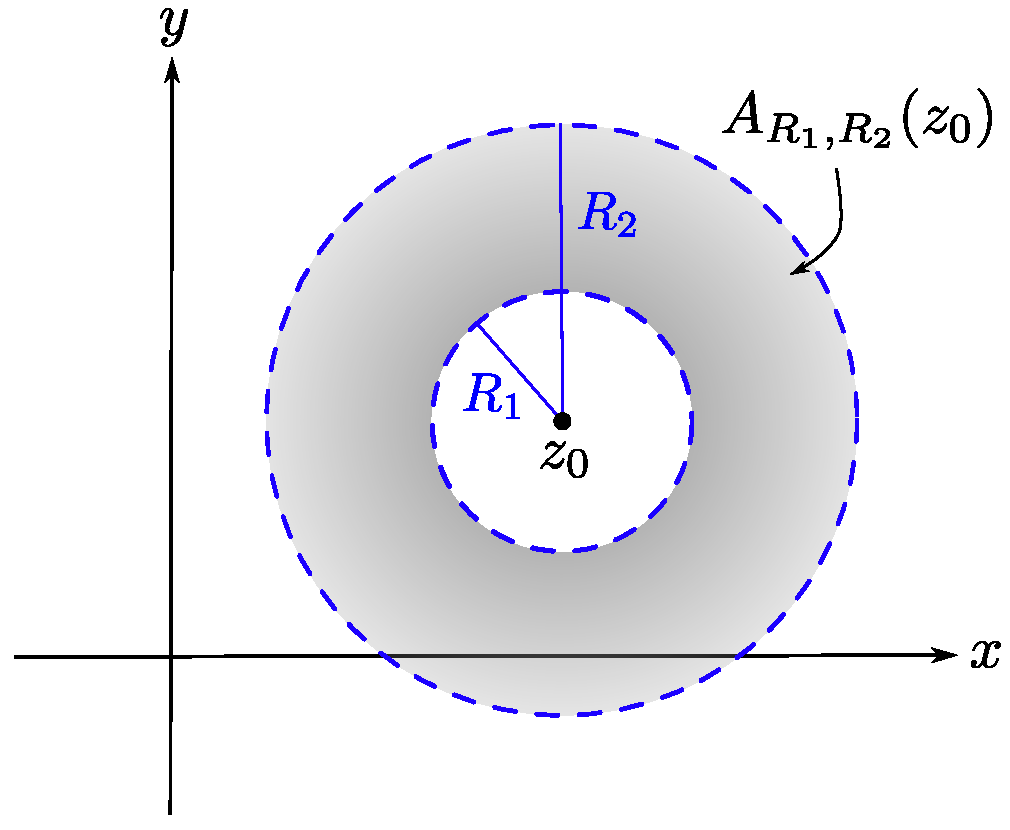
\includegraphics[scale = 0.45]{Figuras/RegionAnular.pdf}
    \caption{Región anular $A_{R_1,R_2}(z_0)$.}
    \label{fig:Annulus}
\end{figure}

\textbf{Observación:} La región anular $A_{R_1,R_2}(z_0)$ se degenera en un disco abierto sin su centro cuando $R_1 = 0$ y $R_2 < \infty$, en un plano sin el centro $z_0$ cuando $R_1 = 0$ y $R_2 = + \infty$, o un plano con un disco centrado en $z_0$ removido cuando $R_1 > 0$ y $R_2 = \infty$.

\begin{teorema}
Si $f$ es analítica en la región anular $A_{R_1,R_2}(z_0)$ donde $0 \leq R_1 < R_2 \leq \infty$. Entonces $f$ tiene una única representación como serie de la forma
\begin{equation}
f(z) = \sum_{n=0}^{\infty} a_n (z-z_0)^n + \sum_{n=1}^{\infty} \frac{b_n}{(z-z_0)^n}, \quad R_1 < |z-z_0| < R_2    \label{SerieLaurent}
\end{equation}

la cual converge absolutamente para $z \in A_{R_1,R_2}(z_0)$ y uniformemente en cada región anular cerrada $\rho_1 \leq |z-z_0| \leq \rho_2$ donde $R_1 < \rho_1$ y $\rho_2 < R_2$. La serie \eqref{SerieLaurent} es llamada \textbf{serie de Laurent} de $f$ y los coeficientes $a_n$ y $b_n$ están dados por:
\begin{align}
    a_n &= \frac{1}{2\pi i} \int_{C_{R}(z_0)} \frac{f(\xi)}{(\xi-z_0)^{n+1}} \,d \xi, \quad n = 0,1,2, \dots \label{CoeLauranet1} \\
    b_n &= \frac{1}{2\pi i} \int_{C_{R}(z_0)} \frac{f(\xi)}{(\xi-z_0)^{-n+1}} \,d \xi, \quad n = 1,2,3, \dots \label{CoeLauranet2}
\end{align}

con $C_{R}(z_0)$ una circunferencia centrada en $z_0$ con radio $R_1 < R < R_2$ orientada positivamente.
\end{teorema}

\begin{proof}

Probaremos que la serie \eqref{SerieLaurent} converge absolutamente y uniformemente en la región anular cerrada $\rho_1 \leq |z-z_0| \leq \rho_2$, donde $R_1 < \rho_1$ y $R_2 < \rho_2$. Fijando $\rho_1$ y $\rho_2$, escogemos $r_1$ y $r_2$ tales que
$$R_1 < r_1 < \rho_1 < \rho_2 < r_2 < R_2$$

y encontramos un $\rho$ tal que $C_{\rho}(z)$ esté contenida en $A_{r_1, r_2}(z_0)$, lo cual es posible porque la región es abierta (ver figura \ref{fig:TeoLaurent}).

\begin{figure}[H]
    \centering
    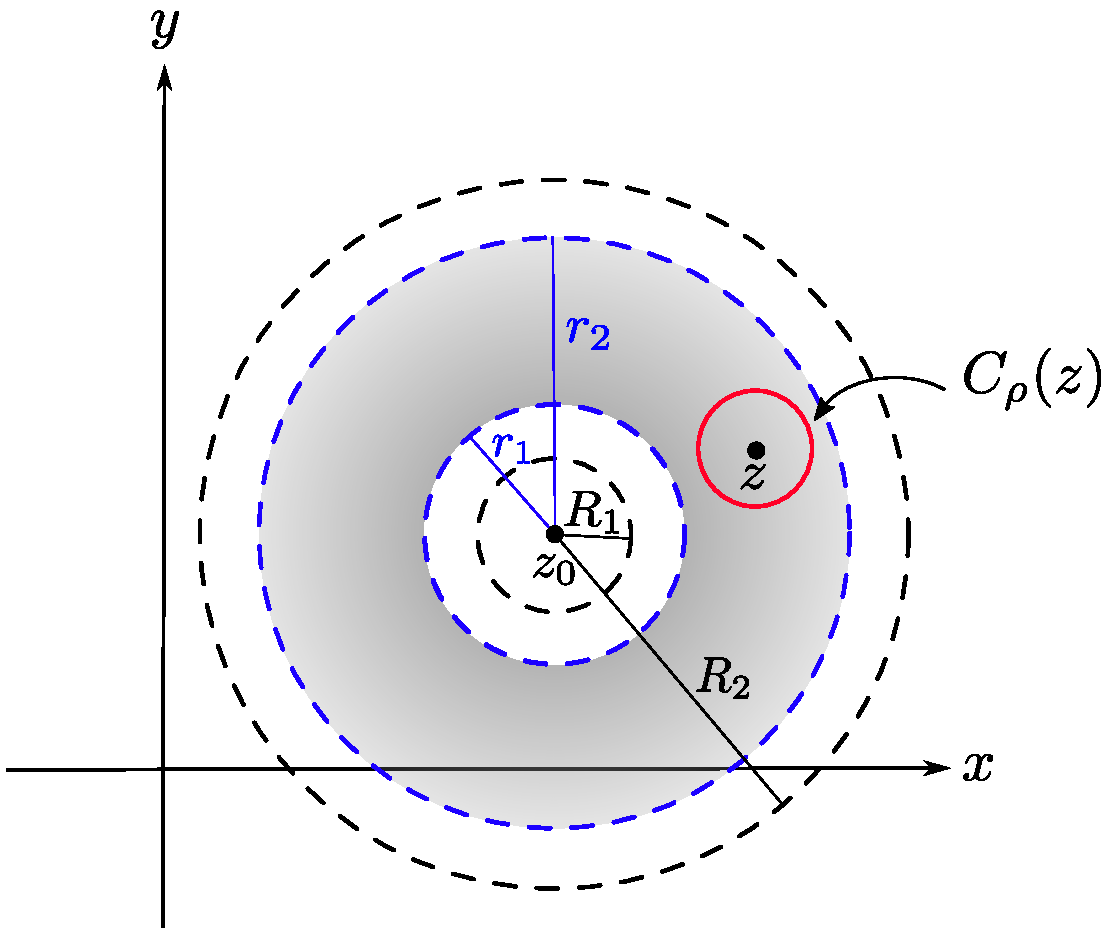
\includegraphics[scale = 0.5]{Figuras/TeoremaLaurent.pdf}
    \caption{Demostración teorema de Laurent.}
    \label{fig:TeoLaurent}
\end{figure}

La función
$$g(\xi) = \frac{f(\xi)}{\xi - z}$$

es analítica en el interior y en la frontera de la región fuera de $C_{\rho}(z)$ y al interior de $A_{r_1,r_2}(z_0)$. Entonces, por el teorema de Cauchy para regiones múltiplemente conexas, tenemos 
$$\frac{1}{2\pi i} \int_{C_{r_2}(z_0)} \frac{f(\xi)}{\xi -z} \,d\xi = \frac{1}{2\pi i} \int_{C_{\rho}(z)} \frac{f(\xi)}{\xi-z} d\xi + \frac{1}{2\pi i} \int_{C_{r_1}(z_0)} \frac{f(\xi)}{\xi - z} \,d\xi,$$

donde todas las circunferencias están orientadas positivamente. Por la fórmula integral de Cauchy, la primera integral al lado derecho de la igualdad es $f(z)$, porque $f$ es analítica dentro de la región anular $A_{R_1,R_2}(z_0)$, más aún al interior de una pequeña vecindad que contiene a $C_{\rho}(z)$. Así,
\begin{equation}
 f(z) = \frac{1}{2\pi i} \int_{C_{r_2}(z_0)} \frac{f(\xi)}{\xi - z} \,d\xi - \frac{1}{2\pi i}  \int_{C_{r_1}(z_0)} \frac{f(\xi)}{\xi - z} \,d\xi. \label{DemLaurent1}
\end{equation}

Para $\xi \in C_{r_2}(z_0)$ y $z$ satisfaciendo $\rho_1 \leq |z-z_0| \leq \rho_2$, tenemos 
$$\frac{|z-z_0|}{|\xi-z_0|} \leq \frac{\rho_2}{r_2} < 1.$$

Luego, podemos escribir
$$\frac{1}{\xi-z} = \frac{1}{\xi - z_0 - (z-z_0)} = \frac{\frac{1}{\xi-z_0}}{1 - \frac{z-z_0}{\xi-z_0}} = \sum_{n=0}^{\infty} \frac{(z-z_0)^n}{(\xi-z_0)^{n+1}}$$

y la serie converge absolutamente y uniformemente en $\xi$ tal que $|\xi-z_0| = r_2$. Entonces, multiplicando por $\frac{1}{2\pi i} f(\xi)$ ambos lados e integrando sobre la circunferencia $C_{r_2}(z_0)$, obtenemos
$$\frac{1}{2\pi i} \int_{C_{r_2}(z_0)} \frac{f(\xi)}{\xi - z} \,d\xi = \sum_{n=0}^{\infty} a_n (z-z_0)^n,$$

donde
\begin{equation}
a_n = \frac{1}{2\pi i} \int_{C_{r_2}(z_0)} \frac{f(\xi)}{(\xi-z_0)^{n+1}} \,d\xi, \quad n = 0,1,2, \dots    \label{DemLaurent2}
\end{equation}

Para la segunda integral al lado derecho de \eqref{DemLaurent1}, tenemos que para $ \xi \in C_{r_1}(z_0)$ y $z$ tales que $\rho_1 \leq |z-z_0| \leq \rho_2$,
$$\frac{|\xi-z_0|}{|z-z_0|} \leq \frac{r_1}{\rho_1} < 1.$$

Luego, podemos escribir
$$\frac{1}{\xi-z} = \frac{1}{\xi - z_0 - (z-z_0)} = \frac{-\frac{1}{z-z_0}}{1 - \frac{\xi-z_0}{z-z_0}} = \sum_{n=0}^{\infty} \frac{-(\xi-z_0)^n}{(z-z_0)^{n+1}} = - \sum_{n=1}^{\infty} \frac{(\xi-z_0)^{n-1}}{(z-z_0)^n}$$

y la serie converge absolutamente y uniformemente en $\xi$ tal que $|\xi-z_0| = r_1$. Entonces, multiplicando por $-\frac{1}{2\pi i} f(\xi)$ ambos lados e integrando sobre la circunferencia $C_{r_1}(z_0)$, obtenemos
\begin{align*}
 -\frac{1}{2\pi i} \int_{C_{r_1}(z_0)} \frac{f(\xi)}{\xi - z} \,d\xi &= \sum_{n=1}^{\infty} \left\{ \frac{1}{2\pi i} \int_{C_{r_1}(z_0)} f(\xi) (\xi - z_0)^{n-1} \,d\xi\right\} \frac{1}{(z-z_0)^n} \\
 &= \sum_{n=1}^{\infty} \frac{b_n}{(z-z_0)^n},
\end{align*}

donde 
\begin{equation}
b_n =  \frac{1}{2\pi i} \int_{C_{r_1}(z_0)} \frac{f(\xi)}{(\xi - z_0)^{-n+1}} \,d\xi, \quad n = 1,2, \dots   \label{DemLaurent3}
\end{equation}

Ahora, para $R \in \,]R_1, R_2[$, por el teorema de deformación, las expresiones \eqref{DemLaurent2} y \eqref{DemLaurent3} son equivalentes a \eqref{CoeLauranet1} y \eqref{CoeLauranet2}, respectivamente.

Finalmente, demostremos la unicidad de la expansión en serie de Laurent. Supongamos que en la región anular $A_{R_1,R_2}(z_0)$ la función $f$ tiene dos series de Laurent:
$$ f(z) = \sum_{n=0}^{\infty} a_n (z-z_0)^n + \sum_{n=1}^{\infty} \frac{b_n}{(z-z_0)^n} = \sum_{n=0}^{\infty} c_n (z-z_0)^n + \sum_{n=1}^{\infty} \frac{d_n}{(z-z_0)^n},$$

las cuales convergen uniformemente en toda subregión anular cerrada de $A_{R_1,R_2}(z_0)$. Multiplicando por $\frac{1}{2\pi i}(z-z_0)^{-k-1}$ ambos lados, con $k \in \mathbb{Z}$, obtenemos que 
\begin{align*}
& \frac{1}{2\pi i}\sum_{n=0}^{\infty} a_n (z-z_0)^{n-k-1} + \frac{1}{2\pi i} \sum_{n=1}^{\infty} b_n (z-z_0)^{-n-k-1} \\
&= \frac{1}{2\pi i} \sum_{n=0}^{\infty} c_n (z-z_0)^{n-k-1} + \frac{1}{2\pi i} \sum_{n=1}^{\infty} d_n (z-z_0)^{-n-k-1}.    
\end{align*}

Ahora, gracias a la convergencia uniforme, integramos término a término las series sobre la circunferencia $C_R(z_0)$ con $R_1 < R < R_2$.
\begin{align*}
&\sum_{n=0}^{\infty}  \frac{1}{2\pi i} \int_{C_R(z_0)}a_n (z-z_0)^{n-k-1} \,dz +  \sum_{n=1}^{\infty} \frac{1}{2\pi i}   \int_{C_R(z_0)} b_n (z-z_0)^{-n-k-1} \,dz \\
&=  \sum_{n=0}^{\infty} \frac{1}{2\pi i} \int_{C_R(z_0)}  c_n (z-z_0)^{n-k-1} \,dz  +  \sum_{n=1}^{\infty} \frac{1}{2\pi i} \int_{C_R(z_0)}  d_n (z-z_0)^{-n-k-1} \,dz.    
\end{align*}

Como
$$\int_{C_R(z_0)} (z-z_0)^m \,dz = \left\{ \begin{array}{cl}
    0, &  \mbox{si} ~ m \neq -1\\
     2\pi i ,& \mbox{si} ~ m = -1
\end{array} \right. ,$$

concluimos que para $k \geq 0$, la integral de cada término de las segundas series y todos los de las primeras, excepto aquel para el que $n = k$, es 0. Por lo tanto,
$$a_k = c_k, \quad k = 0,1,2,\dots$$

y para $k \leq -1$, la integral de todos los términos es 0, excepto aquel de las segundas series con $n = -k$. Por lo tanto,
$$b_{-k} = d_{-k} \Rightarrow b_k = d_k, \quad k = 1,2, \dots$$
\end{proof}

\textbf{Observación:} Si llamamos a $b_n = a_{-n}$, entonces podemos denotar la serie de Laurent por
$$f(z) = \sum_{n= - \infty}^{\infty} a_n (z-z_0)^n$$

con
$$a_n = \frac{1}{2\pi i} \int_{C_R(z_0)} \frac{f(\xi)}{(\xi - z_0)^{n+1}}, \quad n = 0,\pm 1, \pm 2, \dots$$

\begin{ejemplo}
Determinar la serie de Laurent de la función
$$f(z) = \frac{z+1}{z}$$

dentro de la región anular $|z| > 0$.
\\

\textbf{Solución:} Es claro que $f$ es analítica en $\{z \in \mathbb{C}: |z| > 0\} = \mathbb{C} \setminus\{0\}$, luego $f$ admite una representación en serie de Laurent en $\mathbb{C} \setminus\{0\}$. Sea $\gamma$ la circunferencia $|z| = R > 0$, calculemos los coeficientes de la serie:
$$a_n = \frac{1}{2\pi i} \int_{\gamma} \frac{\frac{\xi +1}{\xi}}{\xi^{n+1}} \,d\xi = \frac{1}{2\pi i} \int_{\gamma} \frac{\xi +1}{\xi^{n+2}} \,d\xi = \left\{ \begin{array}{cl}
        1, & \mbox{si}~ n = 0  \\
        0, & \mbox{si}~ n = 1,2, \dots
    \end{array} \right. .$$

y
$$ b_n = \frac{1}{2\pi i} \int_{\gamma} \frac{\frac{\xi +1}{\xi}}{\xi^{-n+1}} \,d\xi = \frac{1}{2\pi i} \int_{\gamma} \frac{\xi +1}{\xi^{-n+2}} \,d\xi = \left\{ \begin{array}{cl}
        1, & \mbox{si}~ n = 1  \\
        0, & \mbox{si} ~n = 2,3, \dots
    \end{array} \right. .
$$

Por lo tanto, la serie de Laurent es
$$\frac{z+1}{z} = 1 + \frac{1}{z}.$$

Sin embargo, note que se obtiene el mismo resultado al simplemente separar la función en dos fracciones, lo cual hace ridículo el cálculo anterior hecho. En general, se recomienda no calcular los coeficientes por medio de las integrales, pues puede resultar bastante laborioso y no trivial. Por esta razón, se sugiere recurrir a series ya conocidas de otras funciones y tener siempre presente la unicidad de las series de Laurent.
\end{ejemplo}

\begin{ejemplo}
Determinar la serie de Laurent de
$$f(z) = \frac{z}{z^2+1}$$

en la región anular $0 < |z-i| < 2$ ($z_0 = i$).
\\

\textbf{Solución:}  Es claro que $f$ es analítica en $A = \{z \in \mathbb{C}: 0< |z-i| < 2\}$, luego $f$ admite una representación en serie de Laurent en $A$. Encontremos esta serie, para ello notemos que
\begin{align}
    \frac{z}{z^2+1} = \frac{z}{(z+i)(z-i)} = \left( \frac{z}{z+i}\right) \frac{1}{z-i} &= \left( \frac{z+i-i}{z+i}\right) \frac{1}{z-i} \nonumber\\
    &=\left(1 - i\frac{1}{z+i}\right) \frac{1}{z-i} \label{EjLaurent1}
\end{align}

Encontremos una expansión en serie de $\frac{1}{z+i}$, con este fin, trabejemos un poco la expresión.
\begin{align*}
    \frac{1}{z+i} = \frac{1}{2i + (z-i)} = \frac{1}{2i} \left( \frac{1}{1+\frac{z-i}{2i}} \right) &= \frac{1}{2i} \left( \frac{1}{1-\left(-\frac{z-i}{2i}\right)} \right) \\
    &= \frac{1}{2i} \sum_{n=0}^{\infty} \left(-\frac{z-i}{2i} \right)^n \\
    &=  \frac{1}{2i} \sum_{n=0}^{\infty} (-1)^n \left(\frac{z-i}{2i} \right)^n \\
    &= \sum_{n=0}^{\infty} (-1)^n \frac{(z-i)^n}{(2i)^{n+1}},
\end{align*}

la cual converge si y sólo si
$$\left| - \frac{z-i}{2i} \right| < 1 \Leftrightarrow |z-i| < 2.$$

Reemplazando en \eqref{EjLaurent1}, tenemos
\begin{align*}
 \frac{z}{z^2+1} = \left( 1 - i \sum_{n=0}^{\infty} (-1)^n \frac{(z-i)^n}{(2i)^{n+1}} \right) \frac{1}{z-i} &= \frac{1}{z-i} - i \sum_{n=0}^{\infty} (-1)^n \frac{(z-i)^{n-1}}{(2i)^{n+1}} \\
 &=  \frac{1}{z-i} - \frac{i}{2i(z-i)} - i\sum_{n=1}^{\infty} (-1)^n \frac{(z-i)^{n-1}}{(2i)^{n+1}} \\
 &= \frac{1}{2(z-i)} - i\sum_{n=0}^{\infty} (-1)^{n+1} \frac{(z-i)^n}{(2i)^{n} (2i)^2} \\
 &=  \frac{1}{2(z-i)} - \frac{i}{4}\sum_{n=0}^{\infty} (-1)^{n} \frac{(z-i)^n}{(2i)^{n}} .
\end{align*}

Notar que de aquí podemos concluir que los coeficientes de la serie de Laurent son:
$$b_n = 0, ~ n > 1; ~ b_1 = \frac{1}{2}; ~ a_n = - \frac{i}{4} \left( -\frac{1}{2i}\right)^n, n\geq 0.$$
\end{ejemplo}

Sabemos que la serie de Laurent converge uniformemente, por lo tanto para $R_1 < |z-z_0| < R_2$, podemos derivar la serie \eqref{SerieLaurent},
$$f'(z) = \sum_{n=1}^{\infty} n a_n (z-z_0)^{n-1} - \sum_{n=1}^{\infty} \frac{n b_n}{(z-z_0)^{n+1}},$$

y la podemos integrar sobre cualquier curva $\gamma$ contenida en $A_{R_1,R_2}(z_0)$,
$$\int_{\gamma} f(z) \,dz = \sum_{n=0}^{\infty} a_n \int_{\gamma} (z-z_0)^n dz + \sum_{n=1}^{\infty} b_n \int_{\gamma} \frac{1}{(z-z_0)^n} \,dz.$$